% Options for packages loaded elsewhere
\PassOptionsToPackage{unicode}{hyperref}
\PassOptionsToPackage{hyphens}{url}
%
\documentclass[
]{book}
\usepackage{lmodern}
\usepackage{amssymb,amsmath}
\usepackage{ifxetex,ifluatex}
\ifnum 0\ifxetex 1\fi\ifluatex 1\fi=0 % if pdftex
  \usepackage[T1]{fontenc}
  \usepackage[utf8]{inputenc}
  \usepackage{textcomp} % provide euro and other symbols
\else % if luatex or xetex
  \usepackage{unicode-math}
  \defaultfontfeatures{Scale=MatchLowercase}
  \defaultfontfeatures[\rmfamily]{Ligatures=TeX,Scale=1}
\fi
% Use upquote if available, for straight quotes in verbatim environments
\IfFileExists{upquote.sty}{\usepackage{upquote}}{}
\IfFileExists{microtype.sty}{% use microtype if available
  \usepackage[]{microtype}
  \UseMicrotypeSet[protrusion]{basicmath} % disable protrusion for tt fonts
}{}
\makeatletter
\@ifundefined{KOMAClassName}{% if non-KOMA class
  \IfFileExists{parskip.sty}{%
    \usepackage{parskip}
  }{% else
    \setlength{\parindent}{0pt}
    \setlength{\parskip}{6pt plus 2pt minus 1pt}}
}{% if KOMA class
  \KOMAoptions{parskip=half}}
\makeatother
\usepackage{xcolor}
\IfFileExists{xurl.sty}{\usepackage{xurl}}{} % add URL line breaks if available
\IfFileExists{bookmark.sty}{\usepackage{bookmark}}{\usepackage{hyperref}}
\hypersetup{
  pdftitle={Forestry Production and Trade in the SWS},
  hidelinks,
  pdfcreator={LaTeX via pandoc}}
\urlstyle{same} % disable monospaced font for URLs
\usepackage{longtable,booktabs}
% Correct order of tables after \paragraph or \subparagraph
\usepackage{etoolbox}
\makeatletter
\patchcmd\longtable{\par}{\if@noskipsec\mbox{}\fi\par}{}{}
\makeatother
% Allow footnotes in longtable head/foot
\IfFileExists{footnotehyper.sty}{\usepackage{footnotehyper}}{\usepackage{footnote}}
\makesavenoteenv{longtable}
\usepackage{graphicx,grffile}
\makeatletter
\def\maxwidth{\ifdim\Gin@nat@width>\linewidth\linewidth\else\Gin@nat@width\fi}
\def\maxheight{\ifdim\Gin@nat@height>\textheight\textheight\else\Gin@nat@height\fi}
\makeatother
% Scale images if necessary, so that they will not overflow the page
% margins by default, and it is still possible to overwrite the defaults
% using explicit options in \includegraphics[width, height, ...]{}
\setkeys{Gin}{width=\maxwidth,height=\maxheight,keepaspectratio}
% Set default figure placement to htbp
\makeatletter
\def\fps@figure{htbp}
\makeatother
\setlength{\emergencystretch}{3em} % prevent overfull lines
\providecommand{\tightlist}{%
  \setlength{\itemsep}{0pt}\setlength{\parskip}{0pt}}
\setcounter{secnumdepth}{5}
\usepackage{booktabs}
\usepackage{longtable}
\usepackage{array}
\usepackage{multirow}
\usepackage{wrapfig}
\usepackage{float}
\usepackage{colortbl}
\usepackage{pdflscape}
\usepackage{tabu}
\usepackage{threeparttable}
\usepackage{threeparttablex}
\usepackage[normalem]{ulem}
\usepackage{makecell}
\usepackage{xcolor}

\title{Forestry Production and Trade in the SWS}
\author{Bruno Caetano Vidigal and Francy Lisboa

Statistician - ESS - Methodological Innovation Team}
\date{2020-04-16}

\begin{document}
\maketitle

{
\setcounter{tocdepth}{1}
\tableofcontents
}
\hypertarget{welcome}{%
\chapter*{\texorpdfstring{\textbf{Welcome}}{Welcome}}\label{welcome}}
\addcontentsline{toc}{chapter}{\textbf{Welcome}}

\textbf{Forestry Production and Trade (FPT)} is migrating its statistical processes into the Corporate Statistical Working System (SWS). This document describes the main institutional actors involved in the migration as well as the FPT - SWS resources (\textbf{code lists}, \textbf{datasets}, \textbf{data tables}) that have been created to support the SWS plugins (R modules) to meet technical unit requirements. Furthermore, the SWS plugins are presented in the form of chapters providing a detailed description of their workflows involving \textbf{input -\textgreater{} processing -\textgreater{} output} as well as results showing whether the modules have lived up to expectations.

\begin{rmdnote}
\textbf{IMPORTANT:} Use the \textbf{Chrome browser} to have a correct
vizualization of HTML outputs in this online document.
\end{rmdnote}

\begin{center}
\includegraphics{images/forestry_cover_book} \end{center}

\hypertarget{preface}{%
\chapter*{\texorpdfstring{\textbf{Preface}}{Preface}}\label{preface}}
\addcontentsline{toc}{chapter}{\textbf{Preface}}

\hypertarget{how-to-use-this-book}{%
\section*{\texorpdfstring{\textbf{How to use this book}}{How to use this book}}\label{how-to-use-this-book}}
\addcontentsline{toc}{section}{\textbf{How to use this book}}

This book contains the entire documentation of the migration of the Forestry Production and Trade statistical processes to the Statistical Working System (SWS).

The chapters are organized by modules.

\begin{table}[H]
\centering\begingroup\fontsize{12}{14}\selectfont

\begin{tabular}{l|l}
\hline
\rowcolor[HTML]{a9c9a7}  Chapter & Description\\
\hline
Ch \textbackslash{}@ref(ForestryFramework) & Provides the framework and entire overview.\\
\hline
Ch \textbackslash{}@ref(ForestryUNECEITTOInputData) & Provides the whole documentation of the module Forestry\_UNECE\_ITTO\_Input\_Data.\\
\hline
Ch \textbackslash{}@ref(ForestryValidationInput) & Provides the whole documentation of the module Forestry\_Validation\_Input.\\
\hline
Ch \textbackslash{}@ref(ForestryCarryForward) & Provides the whole documentation of the module faoswsForestryCarryForward.\\
\hline
Ch \textbackslash{}@ref(faoswsForestryAggregation) & Provides the whole documentation of the module faoswsForestryAggregation..\\
\hline
Ch \textbackslash{}@ref(ForestryValidationAnnualChanges) & Provides the whole documentation of the module ForestryValidationAnnualChanges.\\
\hline
Ch \textbackslash{}@ref(ForestryValidationNegativeConsump) & Provides the whole documentation of the module ForestryValidationNegativeConsumption.\\
\hline
Ch \textbackslash{}@ref(ForestryValidationUnitPrice) & Provides the whole documentation of the module ForestryValidationUnitPrice.\\
\hline
Appendix & Describe all code lists, reference tables (datatables) and data sets.\\
\hline
\end{tabular}
\endgroup{}
\end{table}

\hypertarget{why-to-use-the-sws}{%
\section*{\texorpdfstring{\textbf{Why to use the SWS}}{Why to use the SWS}}\label{why-to-use-the-sws}}
\addcontentsline{toc}{section}{\textbf{Why to use the SWS}}

The Statistical Working System (SWS) is a corporate system that supports data collection, processing and validation, metadata management, and quality assessment of FAO's main statistical domains in line with the Generic Statistical Business Process Model. It has a dual nature -- both technological and statistical -- and for this reason, is developed by two different teams (the IT Division {[}CIO{]} and the Statistics Division {[}ESS{]}). The SWS provides an end-to-end solution for inputting and storing raw data, performing automated statistical processes (e.g.~imputation, validation, etc.), and producing data that are ready for dissemination. Moreover, the reasons why you should use the SWS are:

\begin{itemize}
\tightlist
\item
  The SWS improves data quality by \textbf{centralizing and standardizing} the maintenance of data, classification systems, methodologies, and standards.
\item
  The SWS is \textbf{cost-efficient} in terms of statistical development and functionalities:

  \begin{itemize}
  \tightlist
  \item
    Technical units can adopt methods and even pieces of codes developed for other units: documentation and scripts are open;
  \item
    Users have direct access to some common datasets, thus removing duplication of efforts;
  \item
    New functionalities reflect the requirements of all users and are available to all users, with economies of scale on IT development.
  \end{itemize}
\item
  Users have \textbf{full control of the quality} of the data they are producing:

  \begin{itemize}
  \tightlist
  \item
    Increased use of advanced and semi-automated statistical methods reduce the need for manual interventions and ensure that results are reproducible;
  \item
    Establishment and use of a `basic' set of quality and performance indicators for processes and outputs based on the FAO Statistical Quality Assurance Framework (SQAF);
  \item
    Assessment and publication of quality indicators on a regular basis.
  \end{itemize}
\item
  The SWS ensures \textbf{corporate data consistency} through the adoption of statistical standards. In particular, the SWS

  \begin{itemize}
  \tightlist
  \item
    Facilitates the adoption of corporate standard classifications, metadata and code lists through seamless integration with the corporate Reference Data Management system;
  \item
    Reduces the fragmentation and duplication of sources (e.g.~population data), thus reducing inconsistencies across technical units;
  \item
    Provides flexible tools for a wide range of data collection processes including web data scraping and questionnaire management, thus reducing the duplication of data collection efforts.
  \end{itemize}
\item
  The SWS preserves \textbf{institutional knowledge} by recording the history of data revisions, automating methodology and calculations, and providing end users with unambiguous instructions to follow.
\end{itemize}

Go to the \href{https://hqlqasws1.hq.un.fao.org:8443/sws/}{Statistical Working System} website (restricted access).

\hypertarget{migration-actors}{%
\section*{\texorpdfstring{\textbf{Migration actors}}{Migration actors}}\label{migration-actors}}
\addcontentsline{toc}{section}{\textbf{Migration actors}}

Any migration into the SWS requires the interaction between at least three actors:

\begin{enumerate}
\def\labelenumi{\arabic{enumi}.}
\tightlist
\item
  The \textbf{technical unit} interested in automating either some or all its analytical processes in the SWS. The technical unit can be treated as client demanding services from the counterparts responsible for the implementation of its data and statistical assets in the SWS. Therefore, a successful Forestry Production and Trade migration depends on the coordination between the technical division and other parts. In the Forestry Production and Trade migration to SWS the technical unit is represented by:
\end{enumerate}

\begin{itemize}
\tightlist
\item
  \textbf{Arvydas Lebedys} \emph{Forestry Officer (FOA)}
\item
  \textbf{Roberto Bargigia} \emph{Forestry clerk (FOA)}
\item
  \textbf{Iana Arkhipova} \emph{Statistician (FOA)}
\end{itemize}

\begin{enumerate}
\def\labelenumi{\arabic{enumi}.}
\setcounter{enumi}{1}
\tightlist
\item
  The \textbf{ESS - Methodological Innovation Team} (ESS - SWS) responsible for the implementation and documentation of the required statistical processes. From the ESS - SWS team the focal points are:
\end{enumerate}

\begin{itemize}
\tightlist
\item
  \textbf{Bruno Caetano Vidigal} \emph{Statistician (ESS)}
\item
  \textbf{Francy Lisboa} \emph{Agronomist/Statistician (ESS)}
\item
  \textbf{Luís G. Silva e Silva} \emph{Statistician (ESS)}
\item
  \textbf{Carola Fabi} \emph{Senior Statistician (ESS)}
\end{itemize}

\begin{enumerate}
\def\labelenumi{\arabic{enumi}.}
\setcounter{enumi}{2}
\tightlist
\item
  The \textbf{CIO - SWS} the \textbf{primary backend and frontend maintainer of the SWS} and responsible for the implementation and documentation of non-statistical processes (IT infrastructure). The CIO - SWS team have as interlocutors:
\end{enumerate}

\begin{itemize}
\tightlist
\item
  \textbf{Enrico Anello} \emph{Full Stack Developer (CIO)}
\item
  \textbf{Matteo Terrinoni} \emph{Lead Front End Developer (CIO)}
\item
  \textbf{John Rowell} \emph{Information Technology Officer (CIO)}
\end{itemize}

\hypertarget{ForestryFramework}{%
\chapter{\texorpdfstring{\textbf{Forestry Production and Trade - Framework}}{Forestry Production and Trade - Framework}}\label{ForestryFramework}}

This book focuses on the migration of the Forestry Production and Trade statistical processes to SWS. Therefore, it is important to provide an overview of the statistical value chain carried by FOA. The next sections summarize the Forestry Production and Trade data collection and information management methodology.

\begin{figure}

{\centering 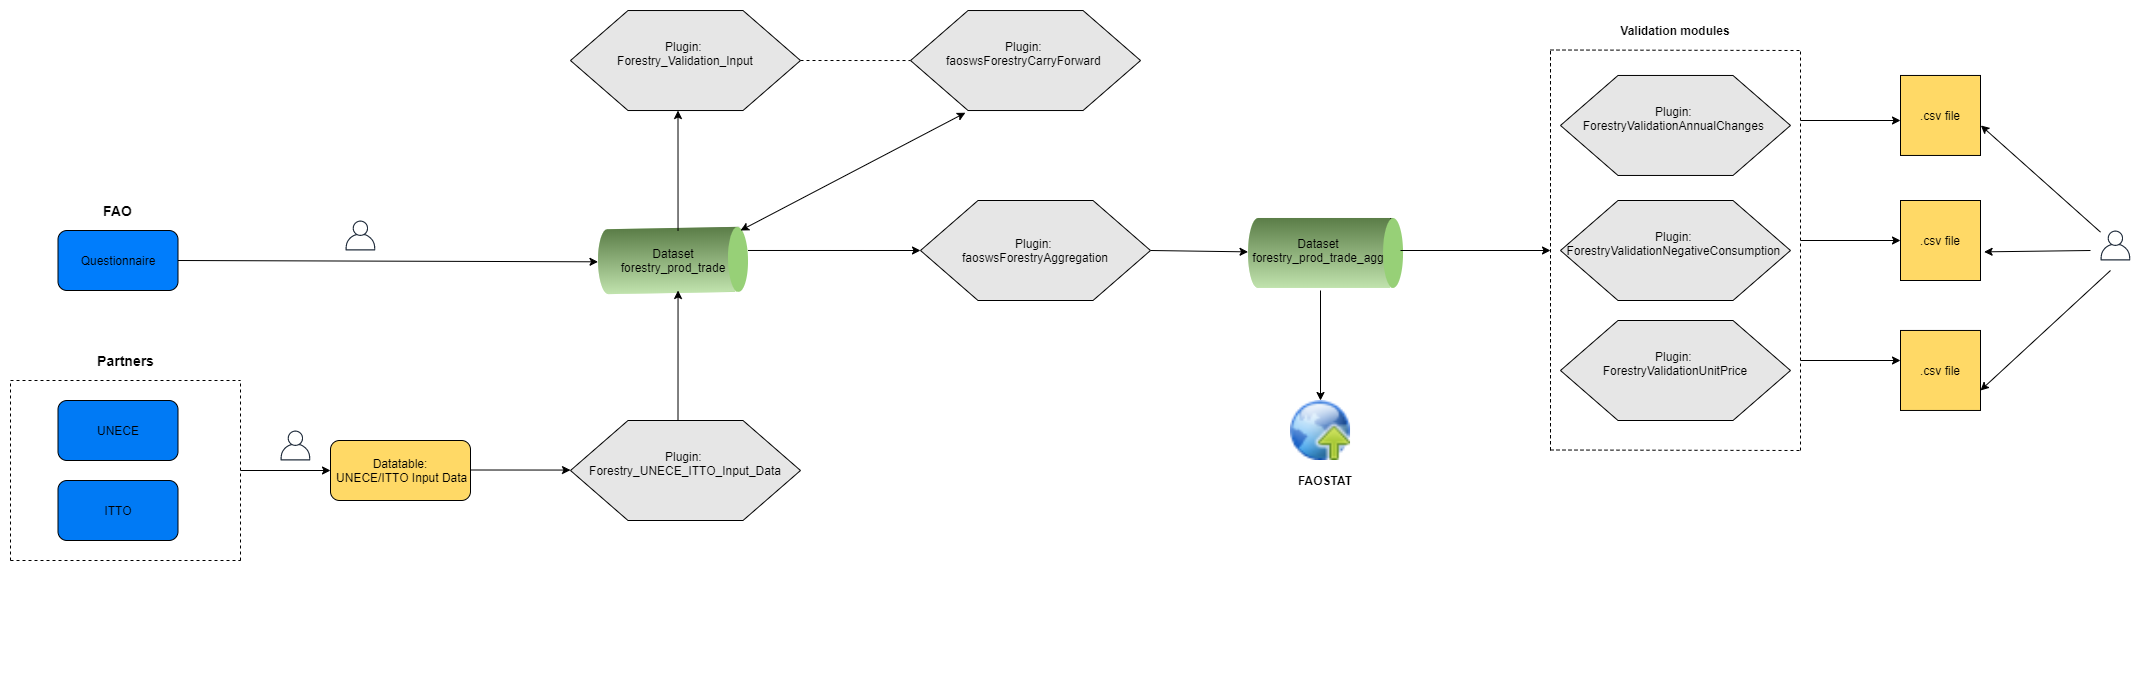
\includegraphics[width=1\linewidth]{images/Forestry_workflow} 

}

\caption{Workflow of the Forestry Production and Trade process}\label{fig:forestryWorkflow}
\end{figure}

\hypertarget{data-collection}{%
\section{\texorpdfstring{\textbf{Data Collection}}{Data Collection}}\label{data-collection}}

The Forestry Production and Trade data collection relies on the \href{http://www.fao.org/forestry/statistics/jfsq/en/}{Joint Forestry Sector Questionnaire distpatch}. The dispatch of the \href{http://www.fao.org/forestry/statistics/jfsq/en/}{same harmonized questionnaire} is carried out by FAO by its international partners:

\begin{itemize}
\tightlist
\item
  \textbf{ITTO} : The \href{https://www.itto.int/}{International Tropical Timber Organization}
\item
  \textbf{Eurostat} : The \href{https://ec.europa.eu/eurostat}{European Statistics}
\item
  \textbf{UNECE} : The \href{http://www.unece.org/info/ece-homepage.html}{United Nations Economic Comission for Europe}
\end{itemize}

FAO sends questionnaires to countries in May/June and the deadline for the first response is September 1st. The partners send out questionnaires between April and June and FAO receives validated data from partners from July to November.

\hypertarget{entering-data}{%
\section{\texorpdfstring{\textbf{Entering Data}}{Entering Data}}\label{entering-data}}

Both data coming from either questionnaires or FAO partners are entered in the SWS by the user through csv files. Once the data are in the system, a validation procedure takes place.

\hypertarget{aggregates}{%
\section{\texorpdfstring{\textbf{Aggregates}}{Aggregates}}\label{aggregates}}

Once the data has been validated, the user is ready to go ahead and generate the aggregates through the module \textbf{faoswsForestryAggregation}. More information about this module is found in the chapter \ref{faoswsForestryAggregation}.

\hypertarget{validationdissemination}{%
\section{\texorpdfstring{\textbf{Validation/Dissemination}}{Validation/Dissemination}}\label{validationdissemination}}

After calculating the aggregates, three modules are ran in order to perform other kinds of validation (annual changes, negative consumption and unit value). More information about these modules are found in the chapters \ref{ForestryValidationAnnualChanges}, \ref{ForestryValidationNegativeConsump} and \ref{ForestryValidationUnitPrice}.
After the step validation, the FOA unit responsible for Forestry Production and Trade can disseminate the data in the FAOSTAT.

\hypertarget{ForestryUNECEITTOInputData}{%
\chapter{\texorpdfstring{\textbf{The Forestry\_UNECE\_ITTO\_Input\_Data module}}{The Forestry\_UNECE\_ITTO\_Input\_Data module}}\label{ForestryUNECEITTOInputData}}

The \textbf{Forestry\_UNECE\_ITTO\_Input\_Data} module is essentially a data harvester. It pulls the raw data provided by partners from the datatable \texttt{UNECE/ITTO\ Input\ Data} and coverts it into a SWS-compliant dataset format. The module deals not only with the data itself, but also with the metadata available.
It is important to note that, while the process described above is automated, the user must upload the \emph{.csv} file format to the datatable \texttt{UNECE/ITTO\ Input\ Data}.

\textbackslash begin\{figure\}

\{\centering 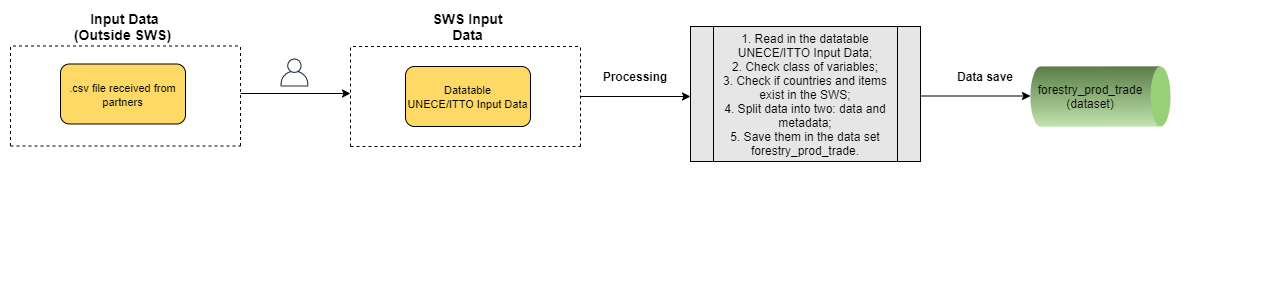
\includegraphics[width=1\linewidth]{images/forestryInputDataUNECE}

\}

\textbackslash caption\{Workflow of the Forestry\_UNECE\_ITTO\_Input\_Data module\}\label{fig:forestryInputData}
\textbackslash end\{figure\}

\hypertarget{steps}{%
\section{\texorpdfstring{\textbf{Steps}}{Steps}}\label{steps}}

The module is straightforward as it checks if the data for countries/items coming from the input data does exist in the \textbf{forestry\_prod\_trade} dataset.

To do so, the module checks the code lists for countries (\textbf{geographicAreaM49}) and for items (\textbf{measuredItemForestry}) as they are used to build the forestry data set. In case there is any inconsistency, a message will pop up in the system warning the user and a input data validation will be needed.

\hypertarget{running-the-module}{%
\section{\texorpdfstring{\textbf{Running the module}}{Running the module}}\label{running-the-module}}

\begin{enumerate}
\def\labelenumi{\arabic{enumi}.}
\item
  Log in the SWS;
\item
  Click on \textbf{New Query};
\item
  Select \textbf{Forestry domain} and \textbf{forestry\_prod\_trade dataset};
\item
  Select whatever geographicAreaM49, measuredElement, measuredItemForestry and timePointYears. After that, run the query;
  \textbackslash begin\{figure\}
\end{enumerate}

\{\centering 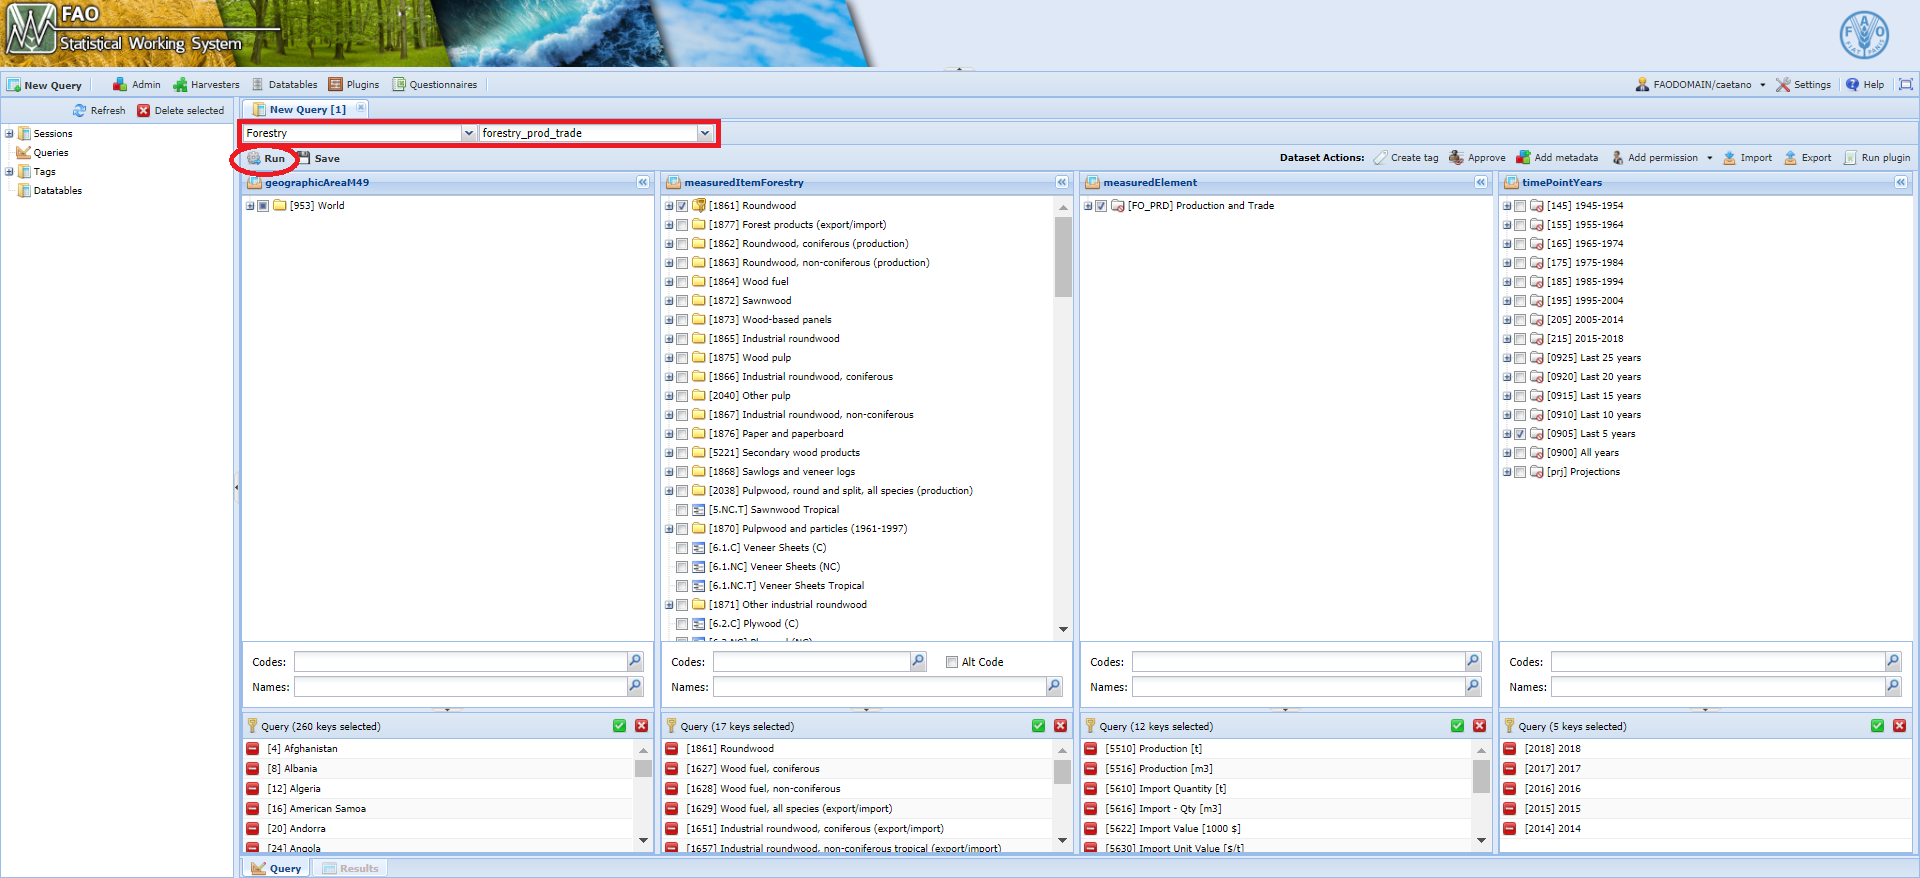
\includegraphics[width=1\linewidth]{images/query_forestry_unece_itto_input_data_plugin}

\}

\caption{Steps 1 to 4}

\label{fig:queryUneceItto}
\textbackslash end\{figure\}
5. Click on \textbf{Run plugin} on the top-right;

\begin{enumerate}
\def\labelenumi{\arabic{enumi}.}
\setcounter{enumi}{5}
\tightlist
\item
  Select the \textbf{Forestry\_UNECE\_ITTO\_Input\_Data} module, choose the \emph{parameters} (Start and End year) and click on \textbf{Run plugin};
\end{enumerate}

\textbackslash begin\{figure\}

\{\centering 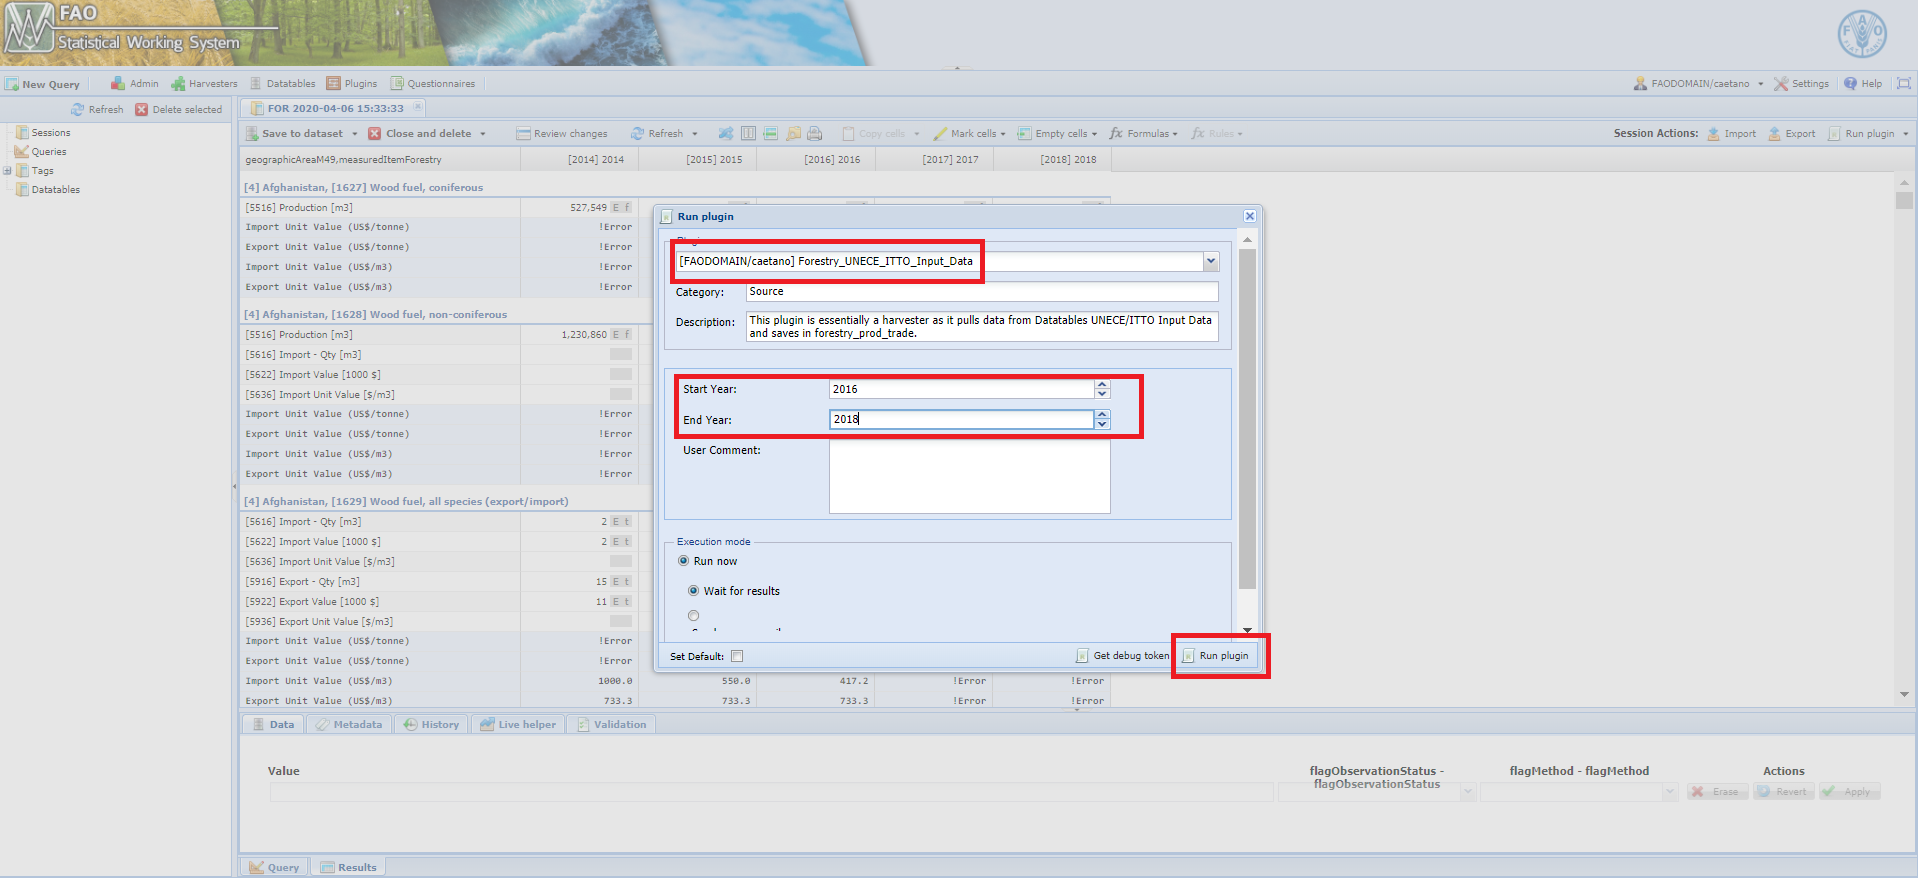
\includegraphics[width=1\linewidth]{images/forestry_select_plugin_unece_itto_input_data}

\}

\textbackslash caption\{Select the Forestry\_UNECE\_ITTO\_Input\_Data plugin and run it\}\label{fig:UneceIttoPlugin}
\textbackslash end\{figure\}
7. Wait for the results to appear in the session;
8. Click on \textbf{Save to dataset}.

\hypertarget{ForestryValidationInput}{%
\chapter{\texorpdfstring{\textbf{The Forestry\_Validation\_Input module}}{The Forestry\_Validation\_Input module}}\label{ForestryValidationInput}}

The \textbf{Forestry\_Validation\_Input} module aims to validate the input data used to calculate aggregates. It plays an important role in detecting inconsistency, if any, as this is the precedent step before the aggregates.

\textbackslash begin\{figure\}

\{\centering 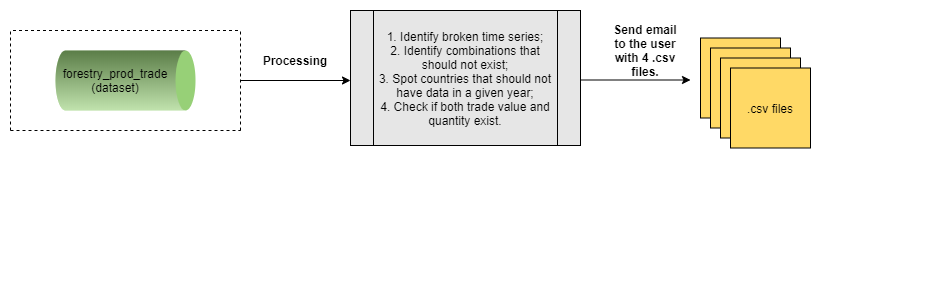
\includegraphics[width=0.85\linewidth]{images/forestryInputDataValidation}

\}

\textbackslash caption\{Workflow of the Forestry\_Validation\_Input module\}\label{fig:forestryInputDataValidation}
\textbackslash end\{figure\}

\hypertarget{steps-1}{%
\section{\texorpdfstring{\textbf{Steps}}{Steps}}\label{steps-1}}

This plugin will be ran over the dataset \textbf{forestry\_prod\_trade} doing the following checks:

\begin{itemize}
\tightlist
\item
  check and identify broken series (e.g.~the country A has data for item I and element E for 1961, 1962, 1963, 1965. In this example, there's a break in the series in 1964);
\item
  check and identify combinations that cannot exist (based on the the datatable \texttt{Forestry\ Product\ Aggregation\ Elements});
\item
  spot countries that should not have data in a given year;
\item
  check inconsistency in the trade data (e.g.~if both trade value and quantity exist).
\end{itemize}

An email will be sent to the user with the four outputs above. This plugin should be tested before the aggregation step. If there's no problem in the dataset, the data is ready to be used as an input to calculate the aggregates.

\hypertarget{running-the-module-1}{%
\section{\texorpdfstring{\textbf{Running the module}}{Running the module}}\label{running-the-module-1}}

\begin{enumerate}
\def\labelenumi{\arabic{enumi}.}
\item
  Log in the SWS;
\item
  Click on \textbf{New Query};
\item
  Select \textbf{Forestry domain} and \textbf{forestry\_prod\_trade dataset};
\item
  Select whatever geographicAreaM49, measuredElement, measuredItemForestry and timePointYears. After that, run the query;
  \textbackslash begin\{figure\}
\end{enumerate}

\{\centering 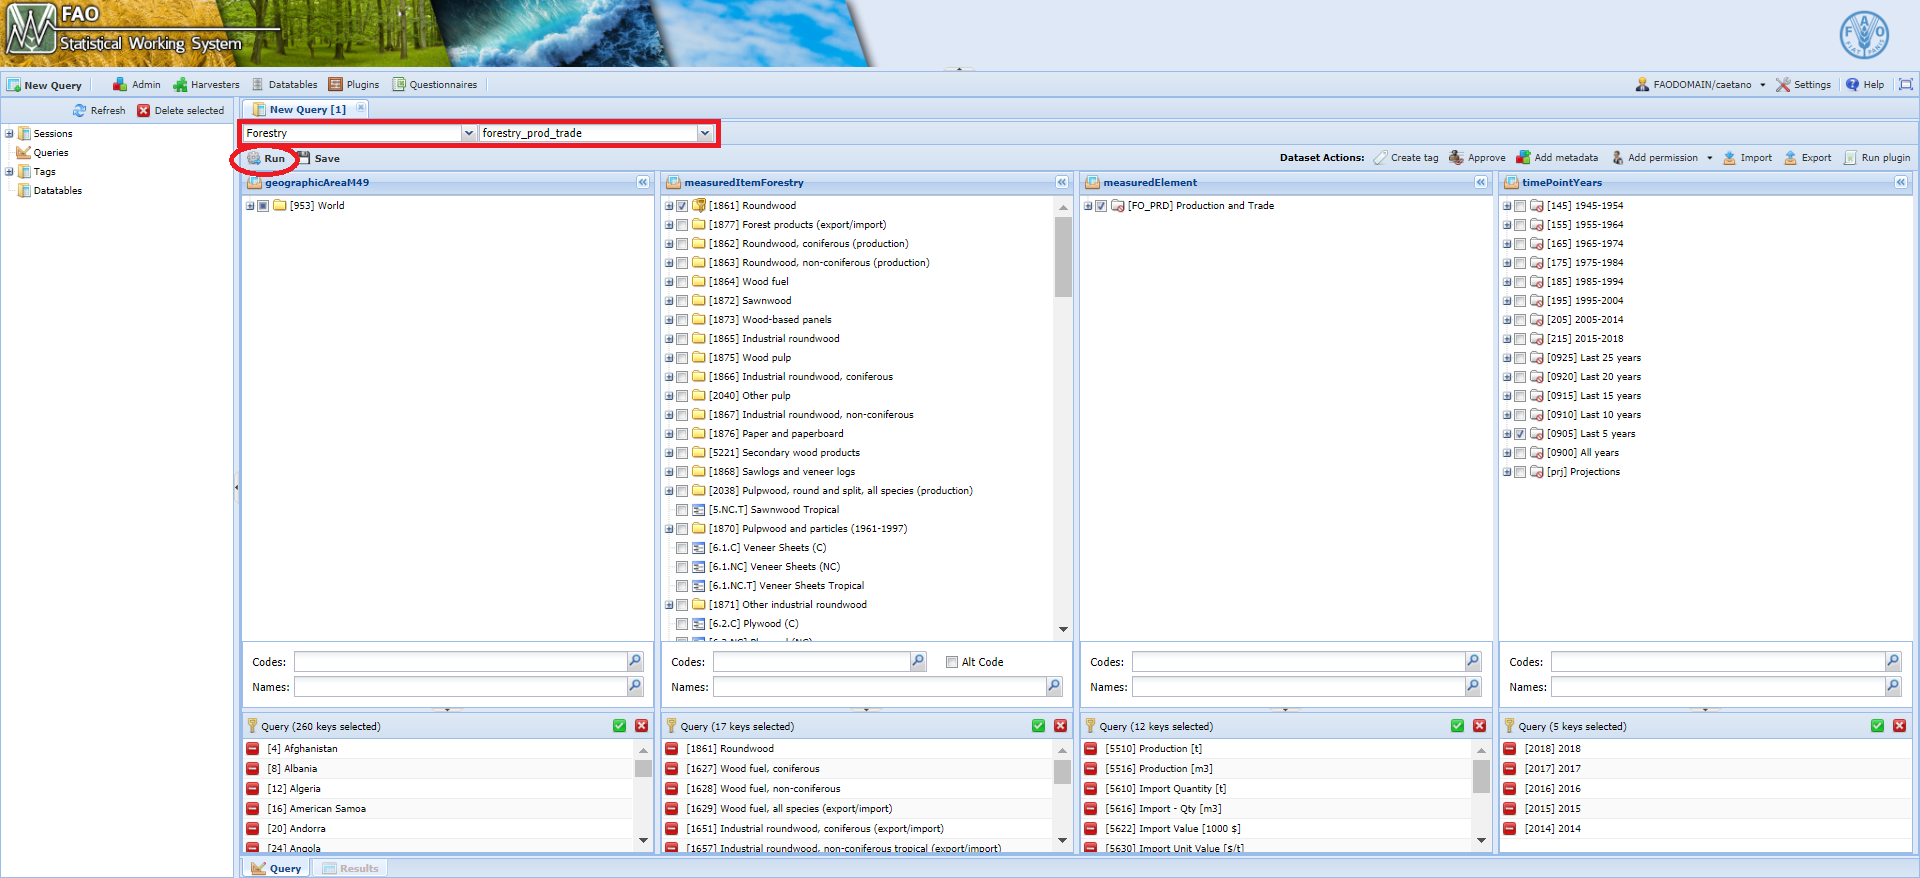
\includegraphics[width=1\linewidth]{images/query_forestry_unece_itto_input_data_plugin}

\}

\caption{Steps 1 to 4}

\label{fig:queryForestryprodtrade}
\textbackslash end\{figure\}
5. Click on \textbf{Run plugin} on the top-right;

\begin{enumerate}
\def\labelenumi{\arabic{enumi}.}
\setcounter{enumi}{5}
\tightlist
\item
  Select the \textbf{Forestry\_Validation\_Input} module, choose the \emph{parameters} (Start and End year) and click on \textbf{Run plugin};
\end{enumerate}

\textbackslash begin\{figure\}

\{\centering 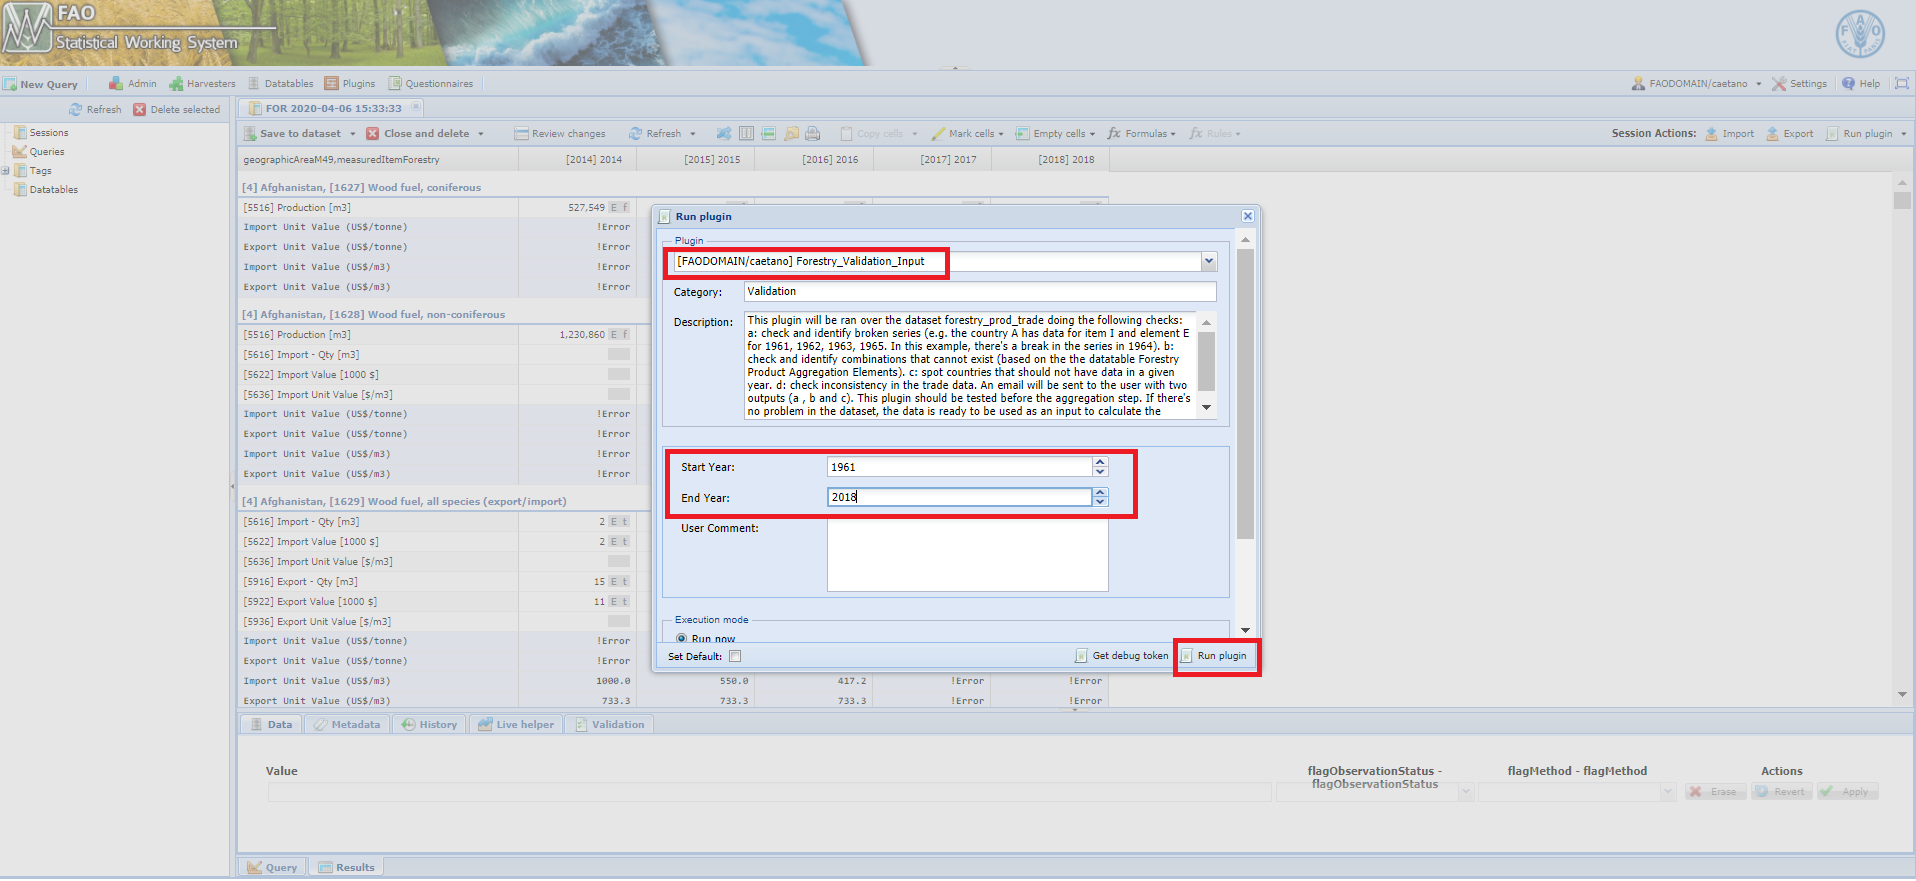
\includegraphics[width=1\linewidth]{images/forestry_input_validation_plugin}

\}

\textbackslash caption\{Select the Forestry\_Validation\_Input plugin and run it\}\label{fig:InputValidationPlugin}
\textbackslash end\{figure\}
7. Wait for the results to appear in the session;
8. Click on \textbf{Save to dataset}.

\hypertarget{ForestryCarryForward}{%
\chapter{\texorpdfstring{\textbf{The faoswsForestryCarryForward module}}{The faoswsForestryCarryForward module}}\label{ForestryCarryForward}}

A step right before calculating the aggregates is to \emph{Carry-Forward} the input data (\textbf{forestry\_prod\_trade} dataset). This step is paramount while the \emph{new data} coming from partners and questionnaires do not arrive. Thus, the whole process does not get stuck and the aggregates are calculated.

\begin{figure}

{\centering 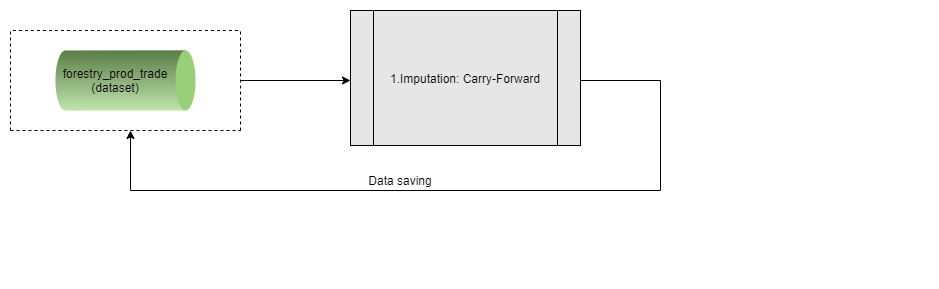
\includegraphics[width=0.85\linewidth]{images/forestryCarryForward} 

}

\caption{Workflow of the faoswsForestryCarryForward module}\label{fig:forestryCarryForward}
\end{figure}

\hypertarget{steps-2}{%
\section{\texorpdfstring{\textbf{Steps}}{Steps}}\label{steps-2}}

The module is straightforward as it just imputes data by the carry-forward method. The module is smart enough to inform the user in case there is already data for the chosen year or if the year in question is too far from the last available year with data.

\hypertarget{running-the-module-2}{%
\section{\texorpdfstring{\textbf{Running the module}}{Running the module}}\label{running-the-module-2}}

\begin{enumerate}
\def\labelenumi{\arabic{enumi}.}
\item
  Log in the SWS;
\item
  Click on \textbf{New Query};
\item
  Select \textbf{Forestry domain} and \textbf{forestry\_prod\_trade dataset};
\item
  Select whatever geographicAreaM49, measuredElement, measuredItemForestry and timePointYears. After that, run the query;
  \textbackslash begin\{figure\}
\end{enumerate}

\{\centering 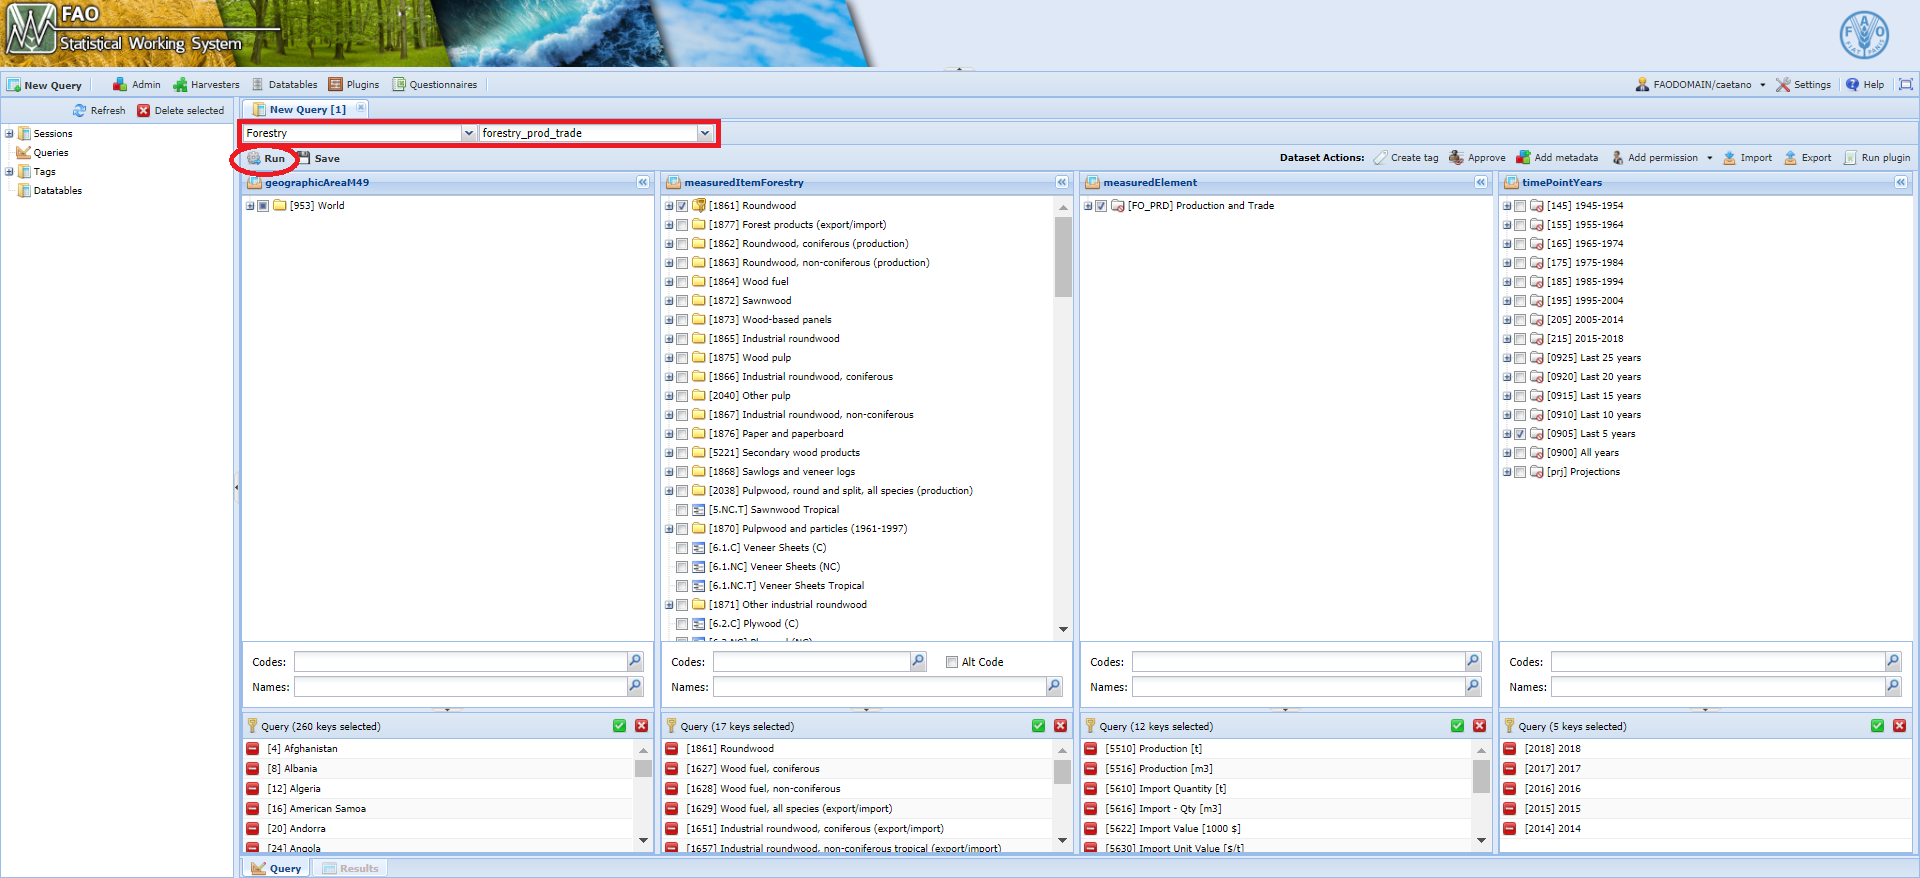
\includegraphics[width=1\linewidth]{images/query_forestry_unece_itto_input_data_plugin}

\}

\caption{Steps 1 to 4}

\label{fig:queryCarryForward}
\textbackslash end\{figure\}
5. Click on \textbf{Run plugin} on the top-right;

\begin{enumerate}
\def\labelenumi{\arabic{enumi}.}
\setcounter{enumi}{5}
\tightlist
\item
  Select the \textbf{faoswsForestryCarryForward} module, choose the \emph{parameter} (Year to impute) and click on \textbf{Run plugin};
\end{enumerate}

\begin{figure}

{\centering 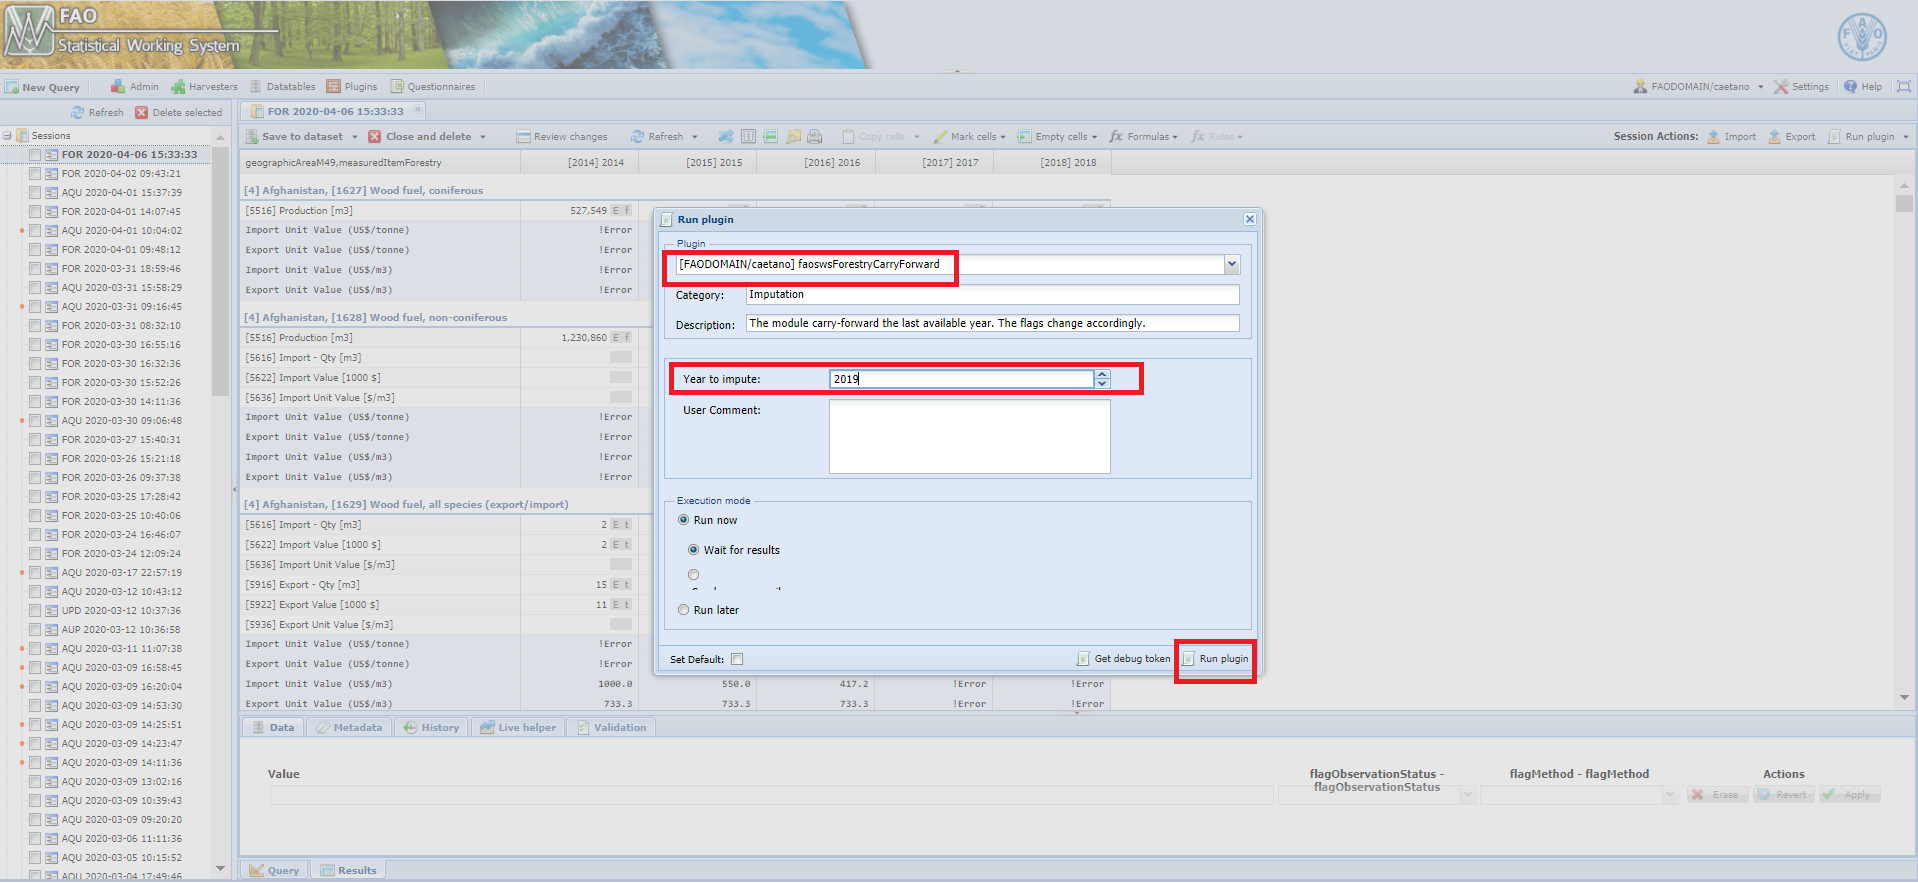
\includegraphics[width=1\linewidth]{images/carry_forward_plugin} 

}

\caption{Select the faoswsForestryCarryForward plugin and run it}\label{fig:CarryForwardPlugin}
\end{figure}

7. Wait for the results to appear in the session;
8. Click on \textbf{Save to dataset}.

\hypertarget{faoswsForestryAggregation}{%
\chapter{\texorpdfstring{\textbf{The faoswsForestryAggregation module}}{The faoswsForestryAggregation module}}\label{faoswsForestryAggregation}}

The module \textbf{faoswsForestryAggregation} comprehend the main step in the \emph{Forestry Production and Trade} process as it calculates the agrgegates by region and item that will be disseminated through \textbf{Faostat}.

\begin{figure}

{\centering \includegraphics[width=0.85\linewidth]{images/faoswsForestryAggregation} 

}

\caption{Workflow of the faoswsForestryAggregation module}\label{fig:faoswsForestryAggregationWorkflow}
\end{figure}

\hypertarget{steps-3}{%
\section{\texorpdfstring{\textbf{Steps}}{Steps}}\label{steps-3}}

The module can be basically split into four parts as below.

\hypertarget{read-in-the-data}{%
\subsection{\texorpdfstring{\textbf{Read in the data}}{Read in the data}}\label{read-in-the-data}}

The module uses the \textbf{forestry\_prod\_trade} dataset as input. According to the technical unit, they will be constantly changing this dataset throughout the data cycle, specially when new data come in or the officers decide to make changes based on their domain knowledge.

\hypertarget{get-regional-aggregation}{%
\subsection{\texorpdfstring{\textbf{Get regional aggregation}}{Get regional aggregation}}\label{get-regional-aggregation}}

After reading in the input dataset, the module geographically aggregates the primary commodities based on FAOSTAT - UNSD M49 mapping. Please, for a full representation of this table consult either the Appendix \ref{tab:m49fsisomapping} or \href{http://www.fao.org/faostat/en/\#data/FO}{this link}.

\hypertarget{get-forestry-commodity-aggregation}{%
\subsection{\texorpdfstring{\textbf{Get Forestry commodity aggregation}}{Get Forestry commodity aggregation}}\label{get-forestry-commodity-aggregation}}

Once a data set with regional aggregate is ready, the module moves to producing commodity aggregations at the national and regional levels.
Since there is an interplay between commodity groups, the module carries the aggregation in tandem, with four commodity groups being aggregated first and then rest of aggregates.

\begin{table}

\caption{\label{tab:tab1}First commodity groups to be calculated by the faoswsForestryAggregation module}
\centering
\fontsize{12}{14}\selectfont
\begin{tabular}[t]{llll}
\toprule
\rowcolor[HTML]{a9c9a7}  CommodityGroup & CommodityGroupName & CommodityCode & CommodityName\\
\midrule
1656 & Chemical wood pulp & 1660 & Chemical wood pulp, sulphite, unbleached\\
1656 & Chemical wood pulp & 1661 & Chemical wood pulp, sulphite, bleached\\
1656 & Chemical wood pulp & 1662 & Chemical wood pulp, sulphate, unbleached\\
1656 & Chemical wood pulp & 1663 & Chemical wood pulp, sulphate, bleached\\
1674 & Printing and writing papers & 1612 & Printing and writing papers, uncoated, wood containing\\
\addlinespace
1674 & Printing and writing papers & 1615 & Printing and writing papers, uncoated, wood free\\
1674 & Printing and writing papers & 1616 & Printing and writing papers, coated\\
1675 & Other paper and paperboard & 1676 & Household and sanitary papers\\
1675 & Other paper and paperboard & 1681 & Wrapping and packaging paper and paperboard\\
1675 & Other paper and paperboard & 1683 & Other paper and paperboard n.e.s.\\
\addlinespace
1681 & Wrapping and packaging paper and paperboard & 1617 & Case materials\\
1681 & Wrapping and packaging paper and paperboard & 1618 & Cartonboard\\
1681 & Wrapping and packaging paper and paperboard & 1621 & Wrapping papers\\
1681 & Wrapping and packaging paper and paperboard & 1622 & Other papers mainly for packaging\\
\bottomrule
\end{tabular}
\end{table}

\hypertarget{get-unit-values}{%
\subsection{\texorpdfstring{\textbf{Get Unit values}}{Get Unit values}}\label{get-unit-values}}

Once the import and export figures are calculated for values and quantity, the unit price, which is the quotient between values and quantity, can be easily calculated for both primary and group commodities at the national and regional levels.

\hypertarget{get-back-the-original-flags}{%
\subsection{\texorpdfstring{\textbf{Get back the original flags}}{Get back the original flags}}\label{get-back-the-original-flags}}

With unit values already in the data sets (national and regional), the last step is to recovery the flags from the original input. Data records added during the processing come either from geographic or commodity aggregation. Therefore, these records have \textbf{``E''} (Aggregation) as flagObservationStatus and \textbf{``s''} (summation) as flagMethod.

\hypertarget{convert-faostat-regions-to-sws-regions}{%
\subsection{\texorpdfstring{\textbf{Convert FAOSTAT regions to SWS regions}}{Convert FAOSTAT regions to SWS regions}}\label{convert-faostat-regions-to-sws-regions}}

The processed regional data set uses FAOSTAT codes for regions. To be able to save the results in the SWS, regions must be converted to SWS regional codes compatible with the \textbf{geographicAreaM49} in the \textbf{forestry\_prod\_trade\_agg} dataset. For this, the module uses the following function.

\hypertarget{binding-national-and-regional-data}{%
\subsection{\texorpdfstring{\textbf{Binding national and regional data}}{Binding national and regional data}}\label{binding-national-and-regional-data}}

Binding national and regional data sets.

\hypertarget{compare-before-and-after-aggregations}{%
\subsection{\texorpdfstring{\textbf{Compare before and after aggregations}}{Compare before and after aggregations}}\label{compare-before-and-after-aggregations}}

As a validation tool, the faoswsForestryAggregation module also needs to return what has changed from the input dataset. The module flags values where the absolute difference between the input dataset and the aggregate dataset is higher than 0.1.

\hypertarget{save-data-in-the-sws-share-drive-and-database}{%
\subsection{\texorpdfstring{\textbf{Save data in the SWS Share Drive and database}}{Save data in the SWS Share Drive and database}}\label{save-data-in-the-sws-share-drive-and-database}}

The data with primary and grouped commodities at the national and regional levels can be accessed by the user as a csv file in the \href{file://hqlprsws1.hq.un.fao.org/sws_r_share/ForestryProdAndTrade/output/faoswsForestryAggregation/}{SWS shared drive}. The full data is saved in the folder \textbf{ForestryProdAndTrade -\textgreater{} output -\textgreater{} faoswsForestryAggregation -\textgreater{} results}, whereas the comparison csv file is saved in the folder \textbf{ForestryProdAndTrade -\textgreater{} output -\textgreater{} faoswsForestryAggregation -\textgreater{} comparisons}. Every time the module runs these files are updated.
In the SWS - database, the data is found in the dataset \textbf{forestry\_prod\_trade\_agg}.

\hypertarget{running-the-module-3}{%
\section{\texorpdfstring{\textbf{Running the module}}{Running the module}}\label{running-the-module-3}}

\begin{enumerate}
\def\labelenumi{\arabic{enumi}.}
\item
  Log in the SWS;
\item
  Click on \textbf{New Query};
\item
  Select \textbf{Forestry domain} and \textbf{forestry\_prod\_trade\_agg dataset};
\item
  Select whatever geographicAreaM49, measuredElement, measuredItemForestry and timePointYears. After that, run the query;
  \textbackslash begin\{figure\}
\end{enumerate}

\{\centering 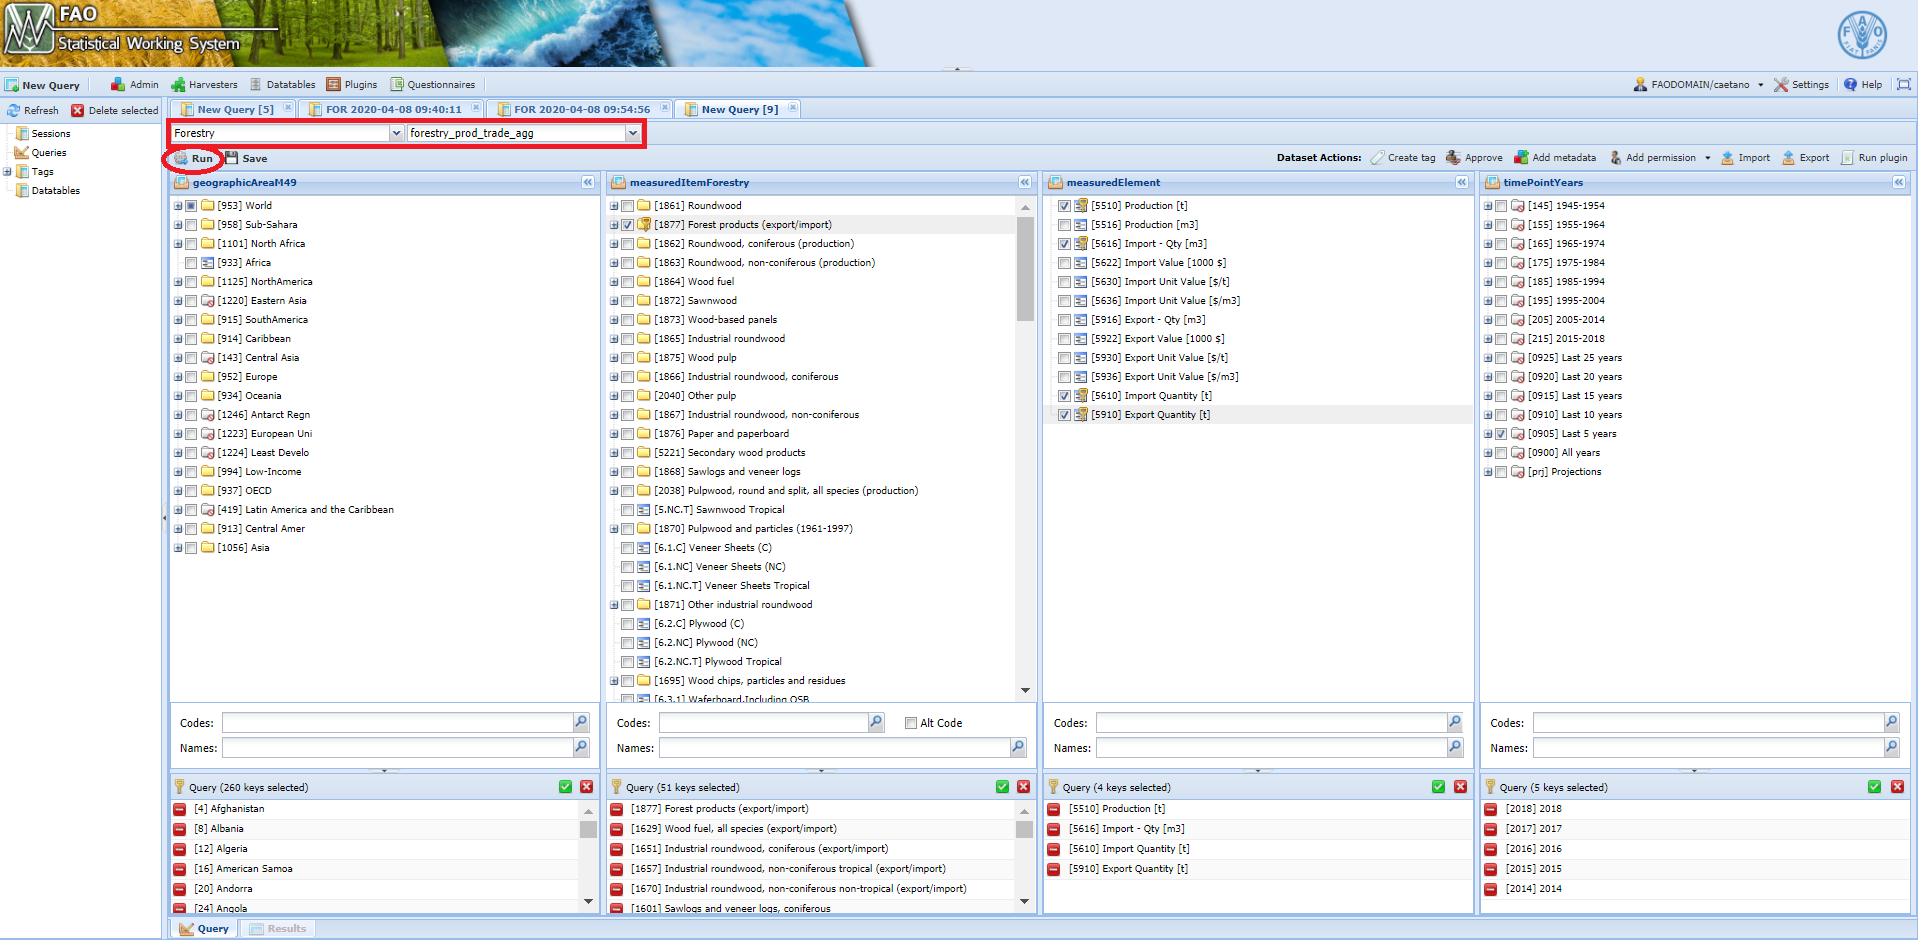
\includegraphics[width=1\linewidth]{images/forestry_prod_trade_agg_query}

\}

\caption{Steps 1 to 4}

\label{fig:queryAggregates}
\textbackslash end\{figure\}

\begin{enumerate}
\def\labelenumi{\arabic{enumi}.}
\setcounter{enumi}{4}
\tightlist
\item
  Select the \textbf{faoswsForestryAggregation} module, choose the \emph{parameters} (Start and End year) and click on \textbf{Run plugin};
\end{enumerate}

\begin{figure}

{\centering 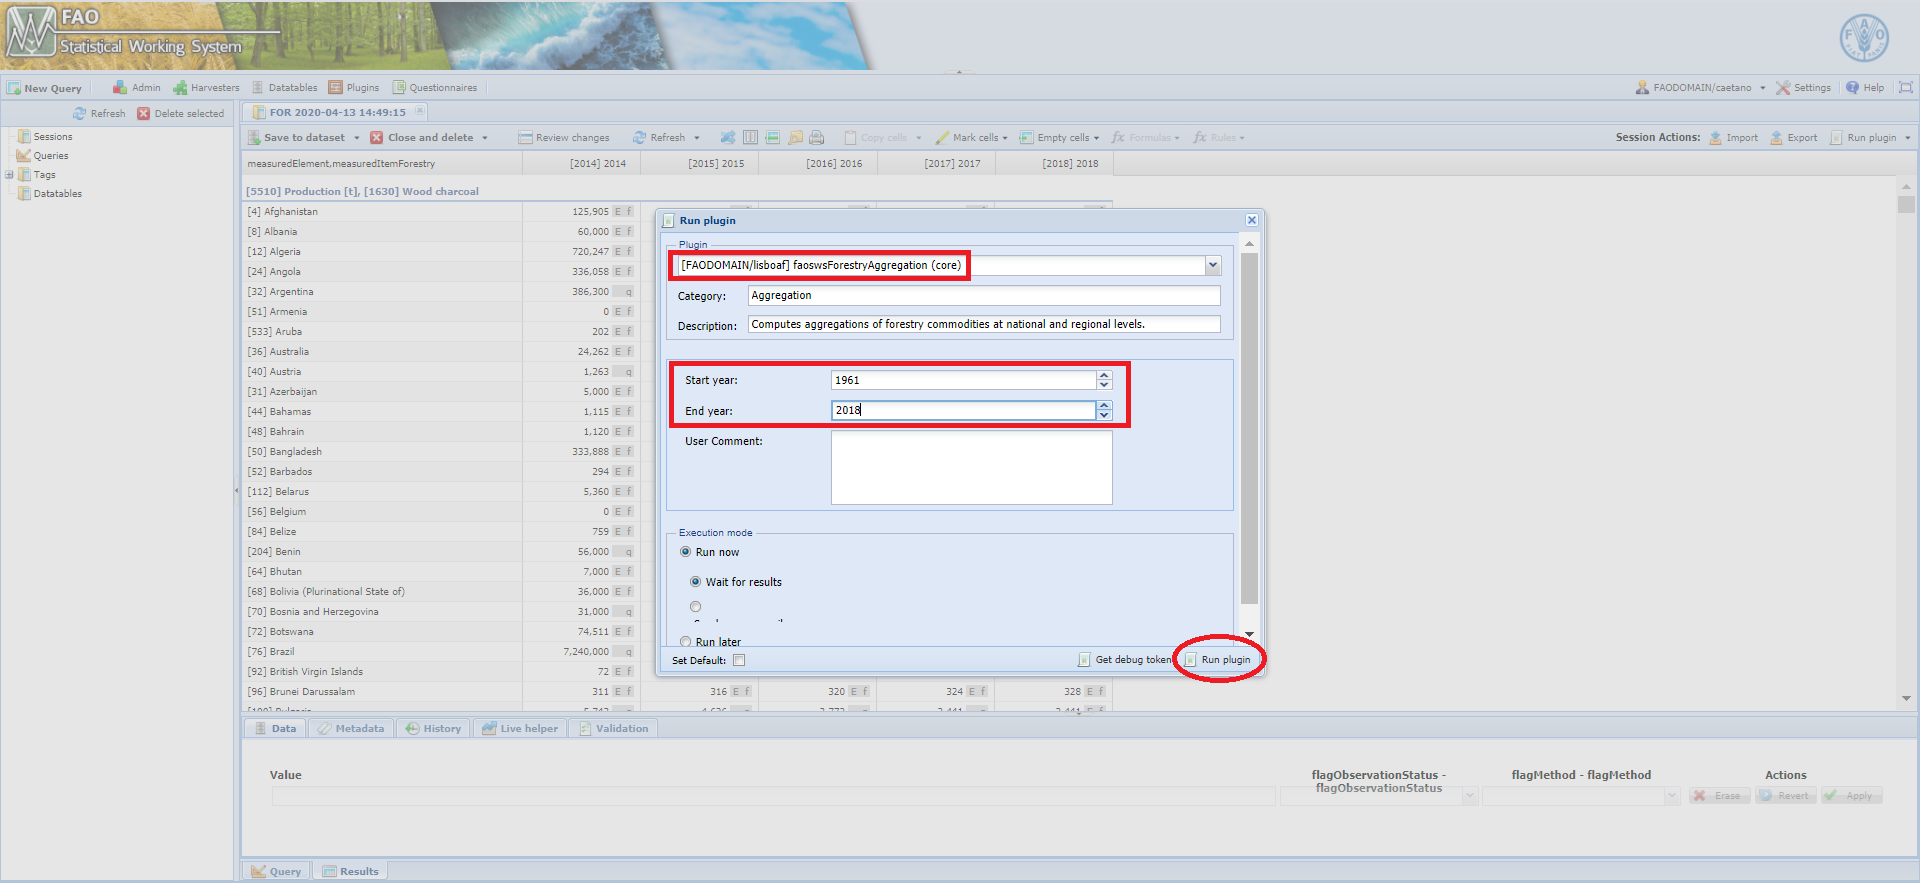
\includegraphics[width=1\linewidth]{images/aggregate_parameters} 

}

\caption{Select the faoswsForestryAggregation plugin and run it}\label{fig:AggregatePlugin}
\end{figure}

6. Wait for a window message to appear in the session: \textbf{ForestryAggregation module ran successfully!!!};
7. Click on \textbf{Save to dataset}.

\hypertarget{ForestryValidationAnnualChanges}{%
\chapter{\texorpdfstring{\textbf{The ForestryValidationAnnualChanges module}}{The ForestryValidationAnnualChanges module}}\label{ForestryValidationAnnualChanges}}

The module \textbf{ForestryValidationAnnualChanges} pulls out records with significant abnormal high annual changes on production, imports and exports according to parameters set by the user.

\begin{figure}

{\centering \includegraphics[width=0.85\linewidth]{images/ForestryValidationAnnualChanges} 

}

\caption{Workflow of the ForestryValidationAnnualChanges module}\label{fig:forestryAnnualChanges}
\end{figure}

\hypertarget{steps-4}{%
\section{\texorpdfstring{\textbf{Steps}}{Steps}}\label{steps-4}}

The module applies simple check in the data. Basically it does the following.

\hypertarget{read-in-data}{%
\subsection{Read in data}\label{read-in-data}}

The module reads data from \textbf{forestry\_prod\_trade\_agg} dataset and from the datatables listed in the figure \ref{fig:ForestryValidationUnitPriceWorkflow}.

\hypertarget{data-filtering}{%
\subsection{Data filtering}\label{data-filtering}}

After pulling the needed data, the module applies filters using the parameters chosen by the user accordingly. The module has two kinds of parameters:

\begin{itemize}
\tightlist
\item
  time range (\emph{start} and \emph{end} year of the process) - \textbf{Start year} and \textbf{End year};
\item
  quantity threshold (minimum quantity analysed) - \textbf{Production Qty threshold}.
\item
  percentage change - \textbf{Percentage Change}.
\end{itemize}

\hypertarget{annual-change-check}{%
\subsection{Annual Change check}\label{annual-change-check}}

At this stage, there are only the target data as the time range and quantity threshold were applied. Therefore, the module verifies if within the remaining data there is any item with an percentage annual change beyond its limits.

\hypertarget{email-the-user}{%
\subsection{Email the user}\label{email-the-user}}

The final step of this module is to email the user with the output.

\hypertarget{running-the-module-4}{%
\section{\texorpdfstring{\textbf{Running the module}}{Running the module}}\label{running-the-module-4}}

\begin{enumerate}
\def\labelenumi{\arabic{enumi}.}
\item
  Log in the SWS;
\item
  Click on \textbf{New Query};
\item
  Select \textbf{Forestry domain} and \textbf{forestry\_prod\_trade\_agg dataset};
\item
  Select whatever geographicAreaM49, measuredElement, measuredItemForestry and timePointYears. After that, run the query;
  \textbackslash begin\{figure\}
\end{enumerate}

\{\centering 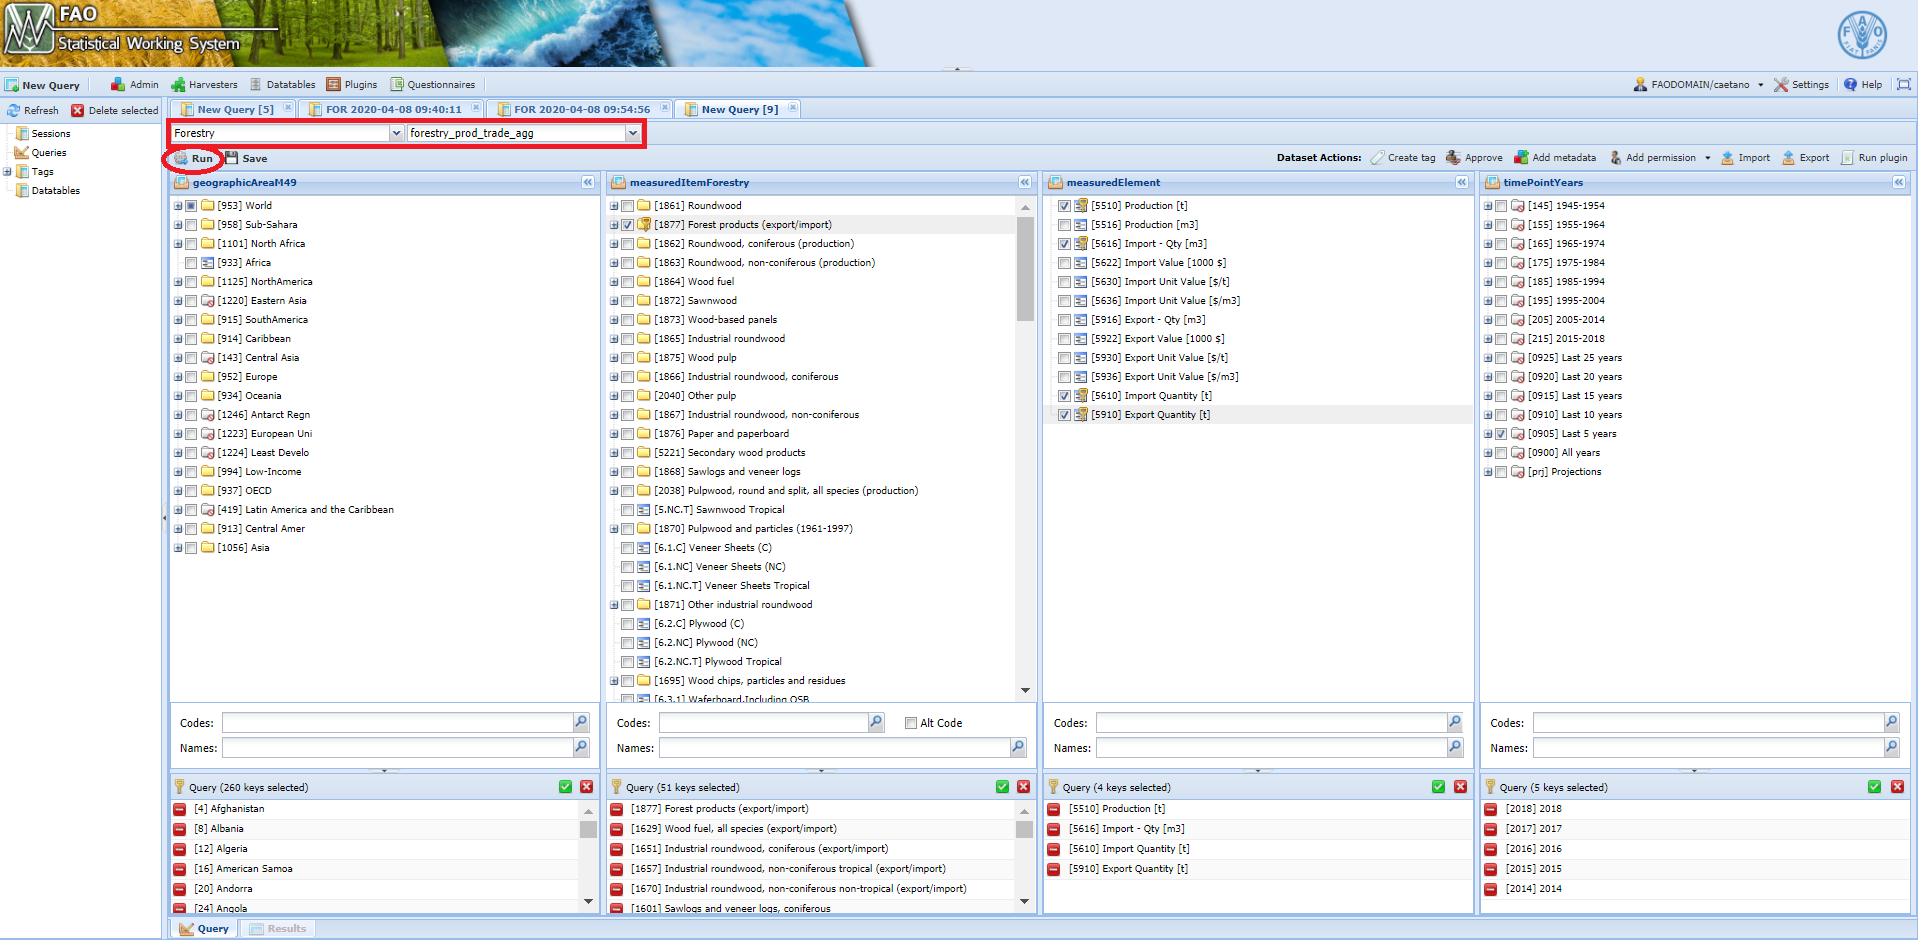
\includegraphics[width=1\linewidth]{images/forestry_prod_trade_agg_query}

\}

\caption{Steps 1 to 4}

\label{fig:queryAnnualChanges}
\textbackslash end\{figure\}

\begin{enumerate}
\def\labelenumi{\arabic{enumi}.}
\setcounter{enumi}{4}
\tightlist
\item
  Select the \textbf{ForestryValidationAnnualChanges} module, choose the \emph{parameters} (Start and End year ; Percentage change ; Production Qty threshold) and click on \textbf{Run plugin};
\end{enumerate}

\begin{figure}

{\centering 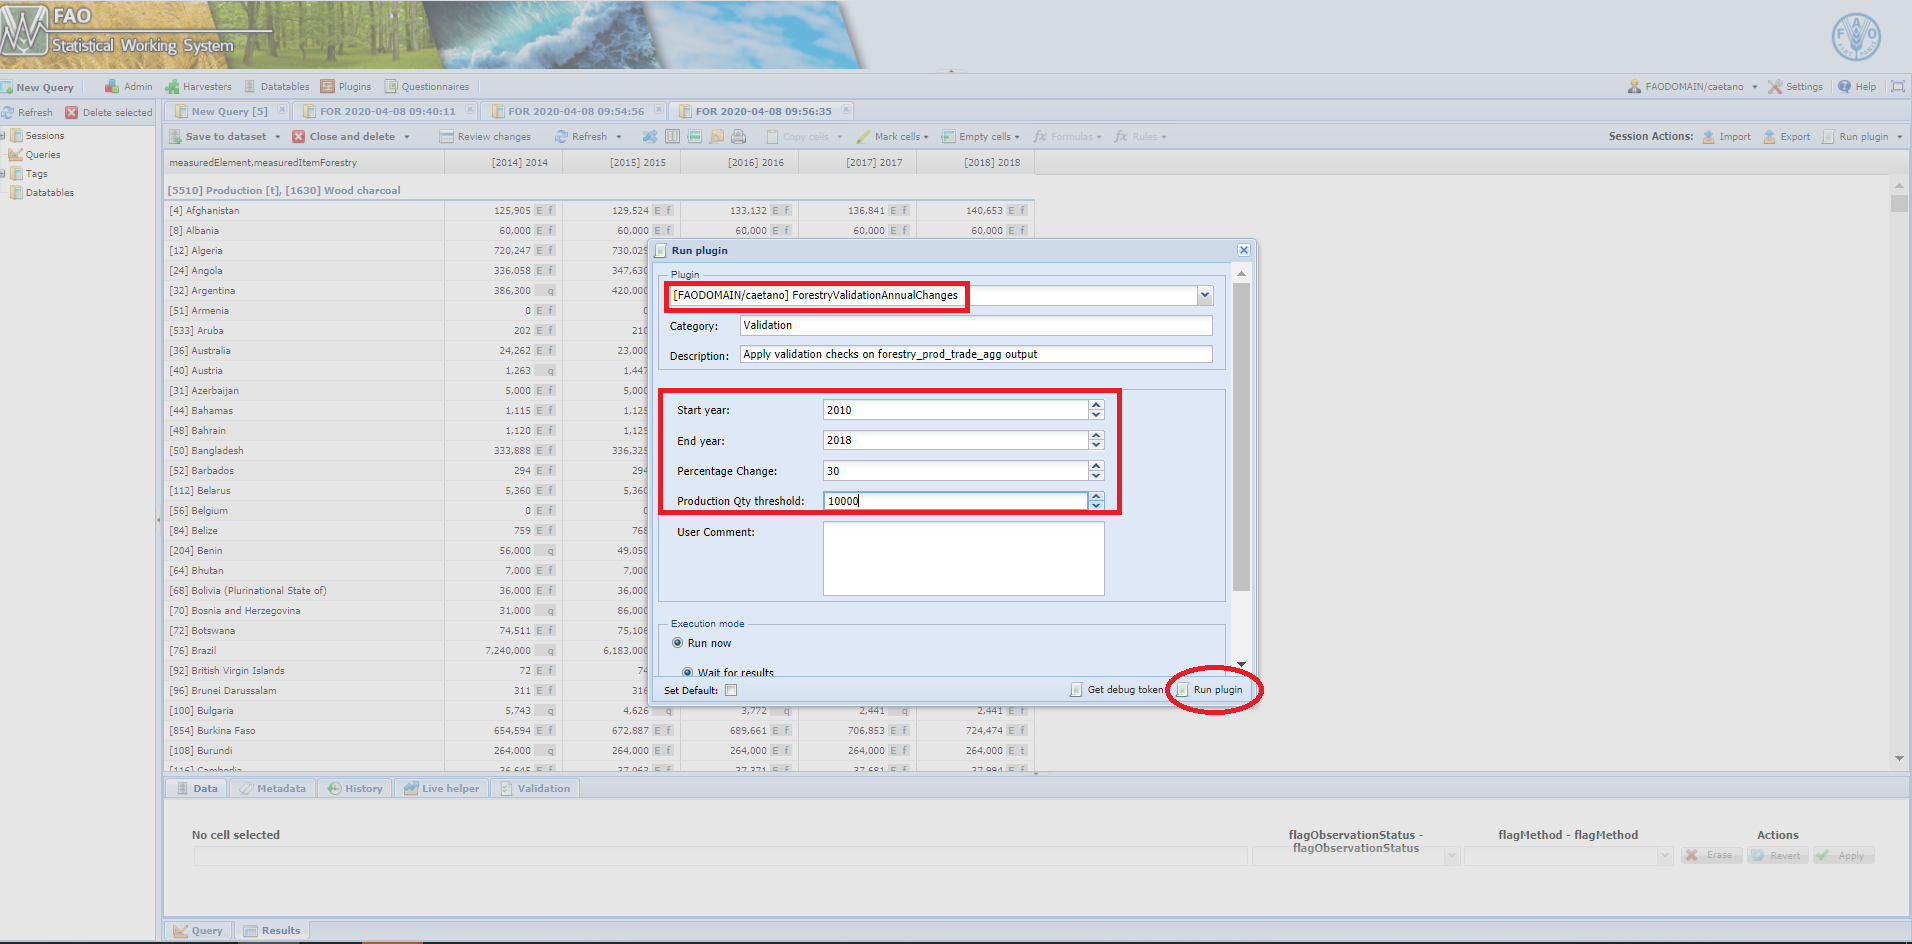
\includegraphics[width=1\linewidth]{images/annual_changes_parameters} 

}

\caption{Select the ForestryValidationAnnualChanges plugin and run it}\label{fig:AnnualChangesPlugin}
\end{figure}

6. Wait for a window message to appear in the session;

\begin{figure}

{\centering 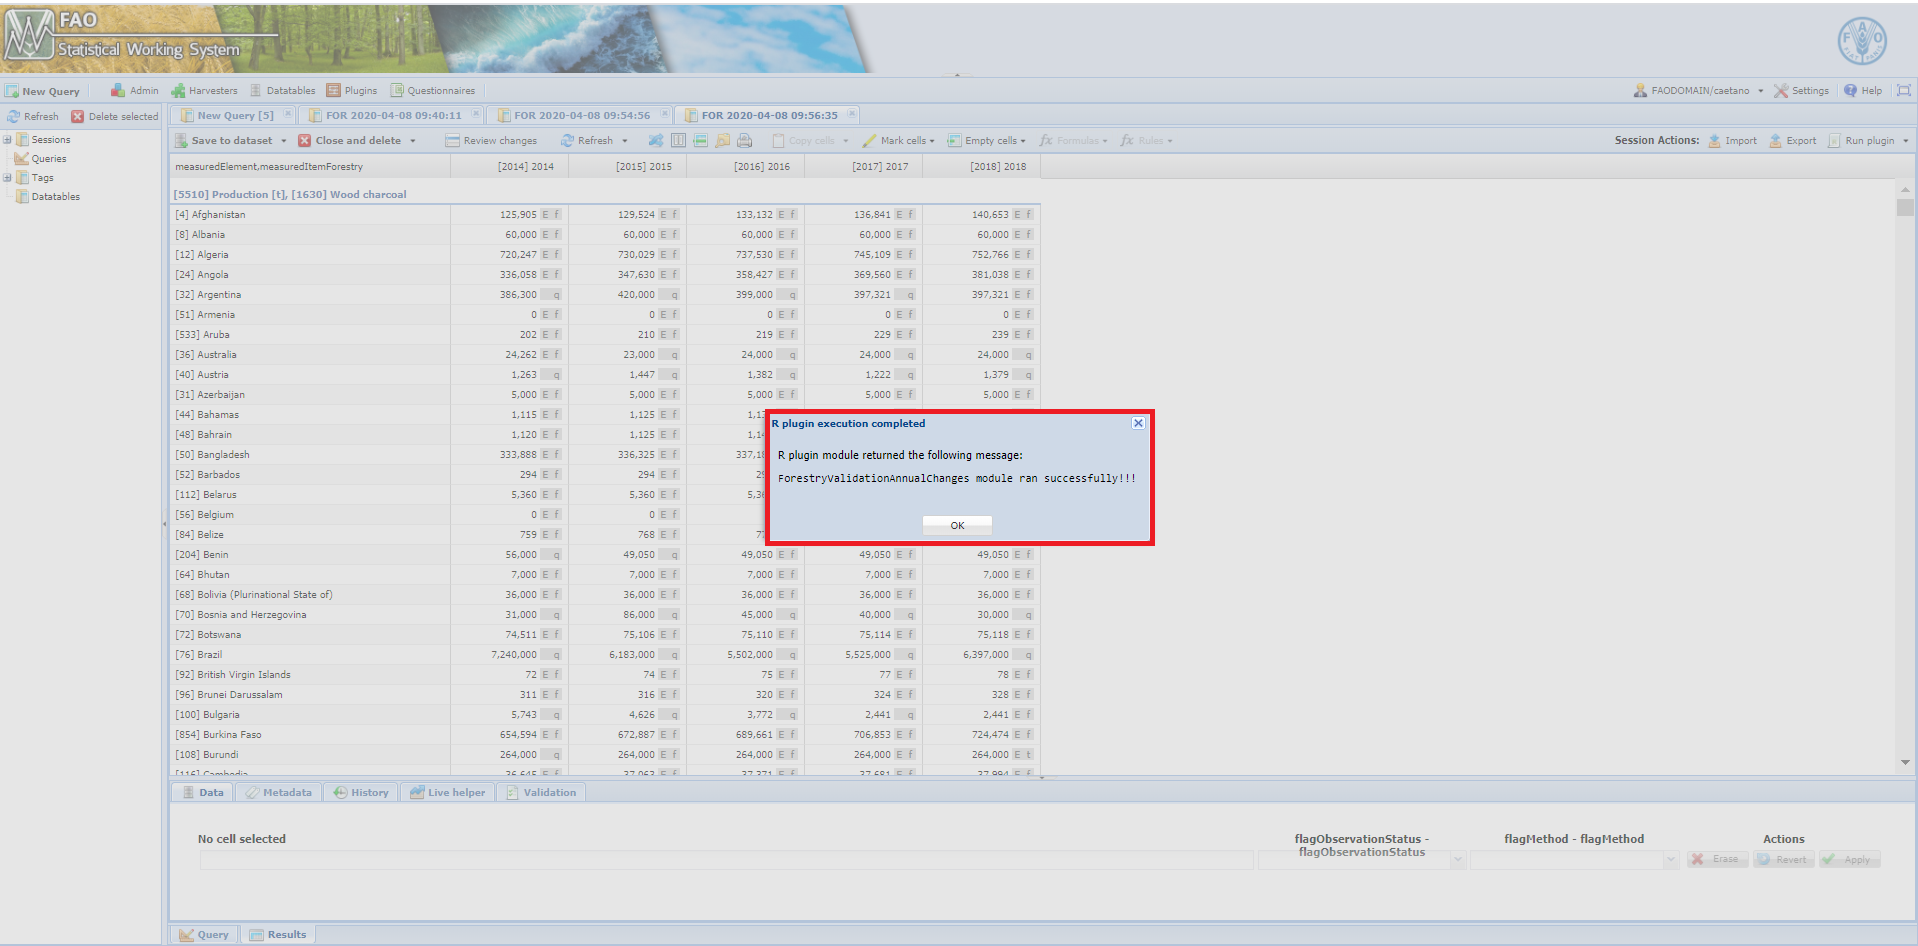
\includegraphics[width=1\linewidth]{images/annual_changes_message} 

}

\caption{ForestryValidationAnnualChanges module ran successfully}\label{fig:AnnualChangesPluginResults}
\end{figure}

\begin{enumerate}
\def\labelenumi{\arabic{enumi}.}
\setcounter{enumi}{6}
\tightlist
\item
  Get your results sent by email.
  \textbackslash begin\{figure\}
\end{enumerate}

\{\centering 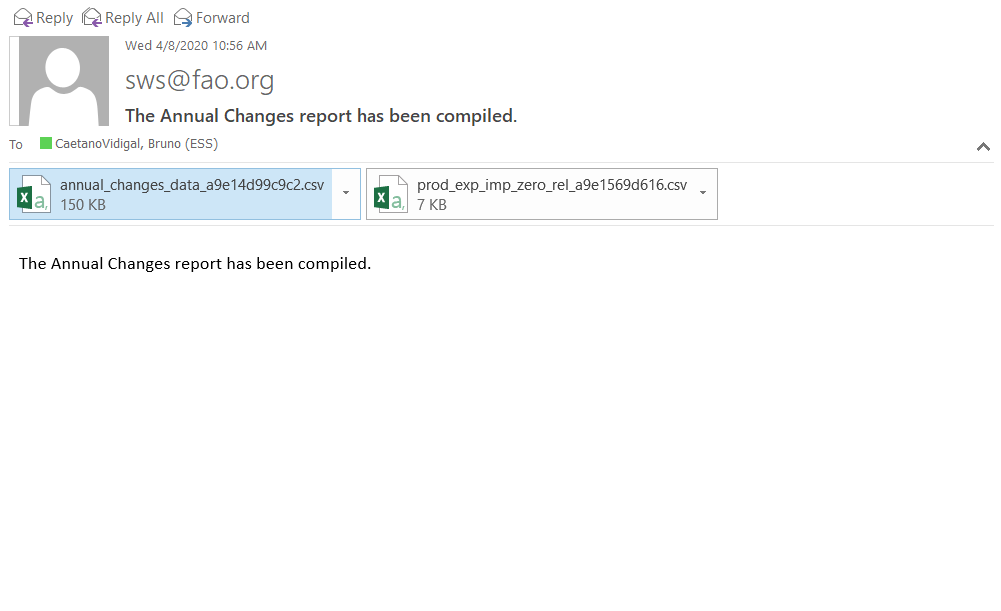
\includegraphics[width=0.8\linewidth]{images/annual_changes_email_sent}

\}

\caption{Email sent to the user with results}

\label{fig:AnnualChangesPluginEmail}
\textbackslash end\{figure\}

\hypertarget{ForestryValidationNegativeConsump}{%
\chapter{\texorpdfstring{\textbf{The ForestryValidationNegativeConsump module}}{The ForestryValidationNegativeConsump module}}\label{ForestryValidationNegativeConsump}}

The module \textbf{ForestryValidationNegativeConsump} is part of the validation procedure before dissemination. As per its name, it carries data validation on the negative consumption, if any. It is up to the user decides the parameters to be used in this phase.

\begin{figure}

{\centering 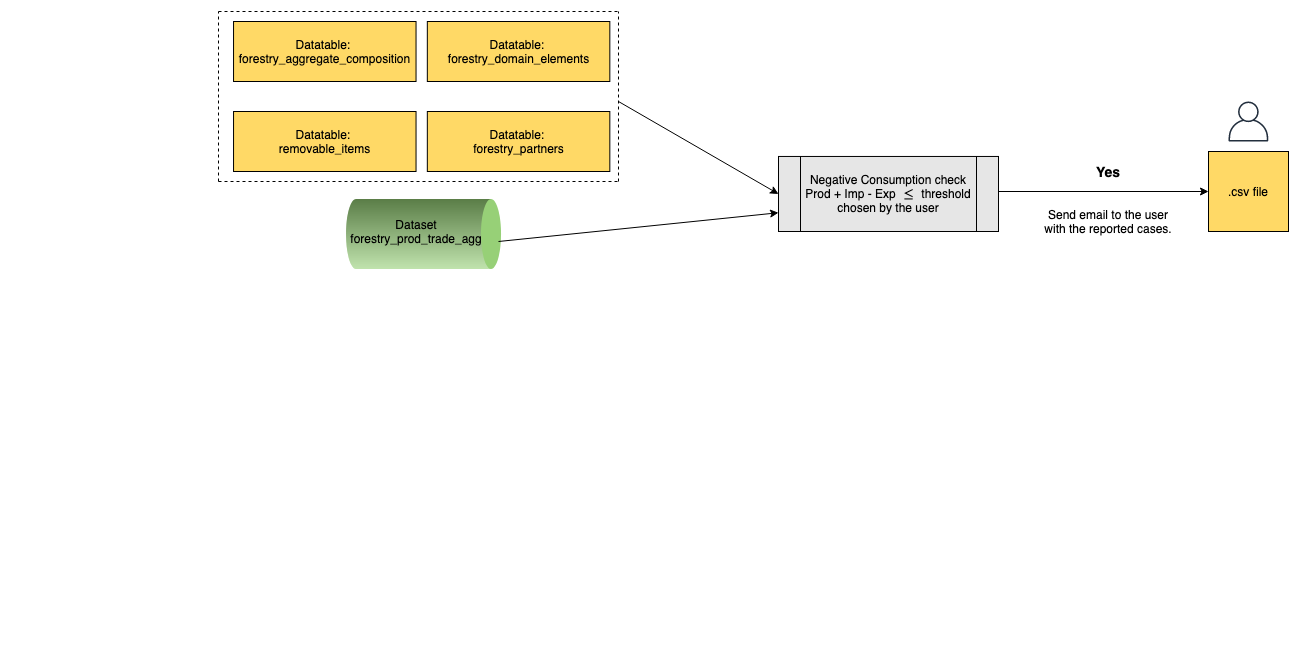
\includegraphics[width=0.85\linewidth]{images/ForestryValidationNegativeConsump} 

}

\caption{Workflow of the ForestryValidationNegativeConsump module}\label{fig:ForestryValidationNegativeConsumpWorkflow}
\end{figure}

\hypertarget{steps-5}{%
\section{\texorpdfstring{\textbf{Steps}}{Steps}}\label{steps-5}}

The module can be basically split into four parts as below.

\hypertarget{read-in-data-1}{%
\subsection{Read in data}\label{read-in-data-1}}

The module reads data from \textbf{forestry\_prod\_trade\_agg} dataset and from the datatables listed in the figure \ref{fig:ForestryValidationNegativeConsumpWorkflow}.

\hypertarget{data-filtering-1}{%
\subsection{Data filtering}\label{data-filtering-1}}

After pulling the needed data, the module applies filters using the parameters chosen by the user accordingly. The module has two kinds of parameters:

\begin{itemize}
\item
  time range (\emph{start} and \emph{end} year of the process) - \textbf{Start year} and \textbf{End year};
\item
  negative consumption threshold - \textbf{Negative consumption threshold}. For instance, in this case if the user chooses \texttt{-1000}, the module will filter the time series that contain at least one data point with a \texttt{Consumption\ \textless{}=\ -1000}. For the sake of clarification, Consumption is definied as below:

  \begin{itemize}
  \tightlist
  \item
    \textbf{Consumption = Production + Imports - Exports}
  \end{itemize}
\end{itemize}

\hypertarget{negative-consumption-check}{%
\subsection{Negative consumption check}\label{negative-consumption-check}}

At this stage, the module performs the \emph{Negative Consumption} check over the data by using the parameter chosen by the user.

\hypertarget{email-the-user-1}{%
\subsection{Email the user}\label{email-the-user-1}}

The final step of this module is to email the user with one \emph{.csv} file - negative consumption report.

\hypertarget{running-the-module-5}{%
\section{\texorpdfstring{\textbf{Running the module}}{Running the module}}\label{running-the-module-5}}

\begin{enumerate}
\def\labelenumi{\arabic{enumi}.}
\item
  Log in the SWS;
\item
  Click on \textbf{New Query};
\item
  Select \textbf{Forestry domain} and \textbf{forestry\_prod\_trade\_agg dataset};
\item
  Select whatever geographicAreaM49, measuredElement, measuredItemForestry and timePointYears. After that, run the query;
  \textbackslash begin\{figure\}
\end{enumerate}

\{\centering 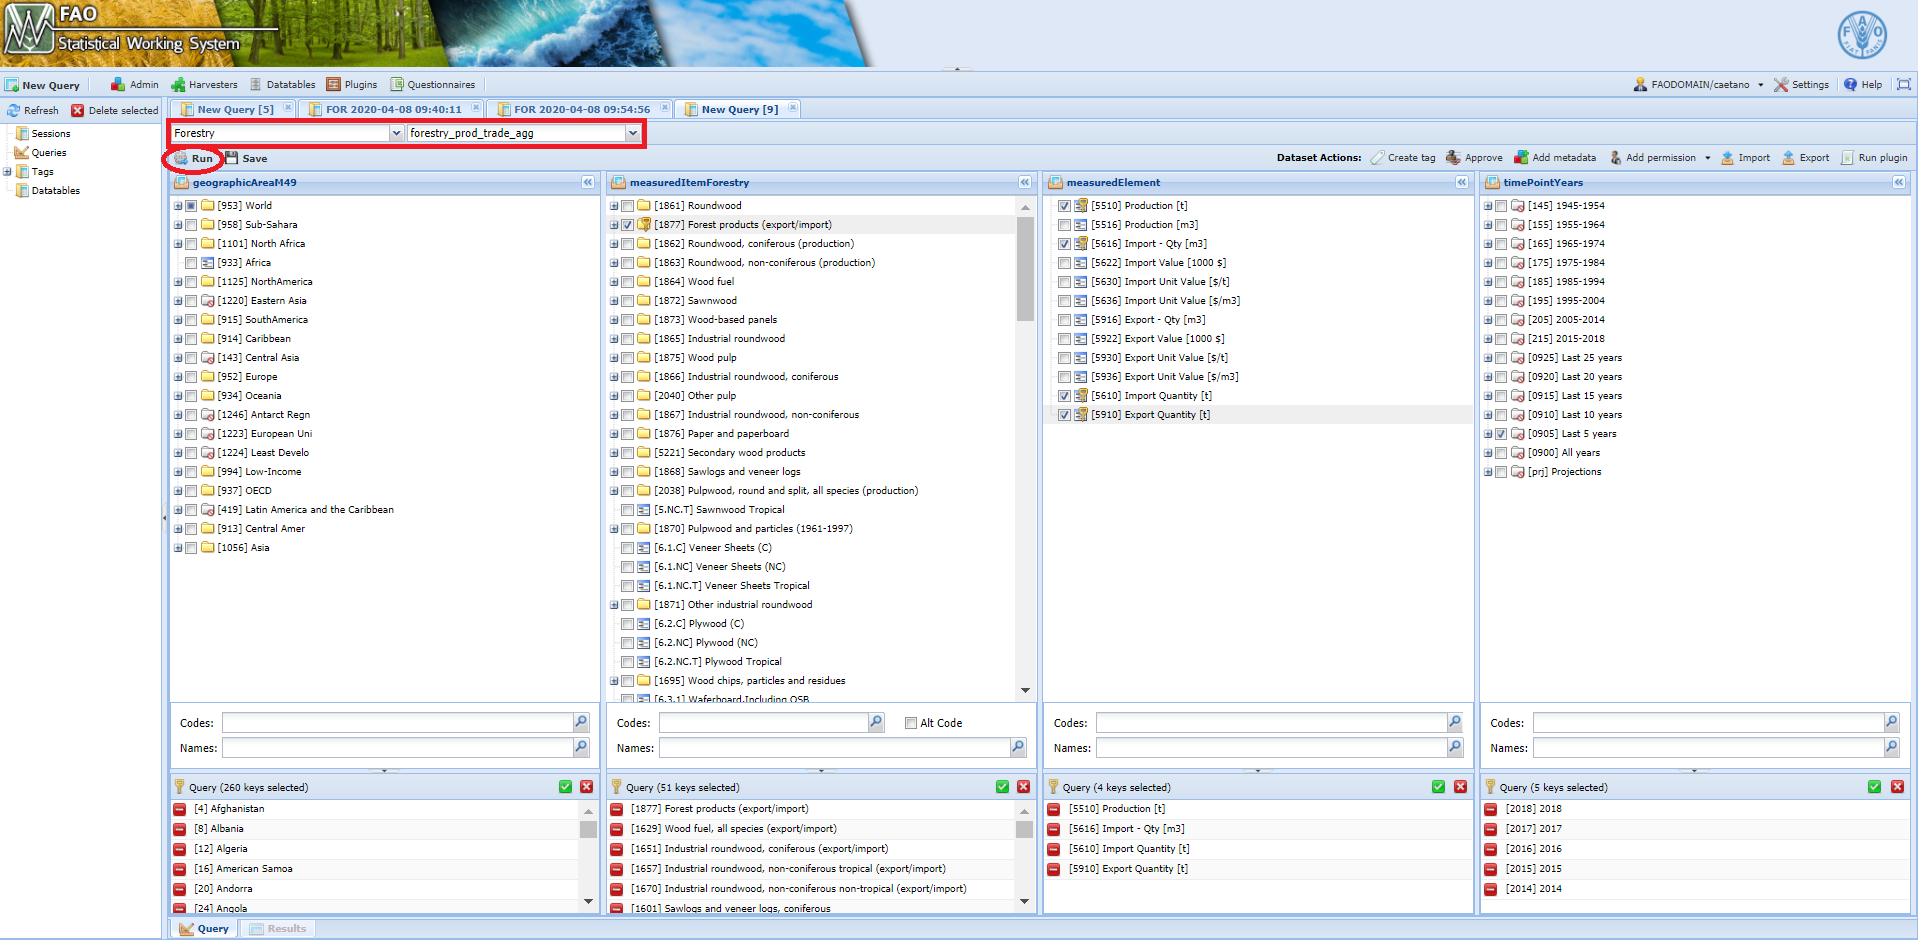
\includegraphics[width=1\linewidth]{images/forestry_prod_trade_agg_query}

\}

\caption{Steps 1 to 4}

\label{fig:queryNegConsump}
\textbackslash end\{figure\}

\begin{enumerate}
\def\labelenumi{\arabic{enumi}.}
\setcounter{enumi}{4}
\tightlist
\item
  Select the \textbf{ForestryValidationNegativeConsump} module, choose the \emph{parameters} (Start and End year ; Negative Consumption threshold) and click on \textbf{Run plugin};
\end{enumerate}

\begin{figure}

{\centering 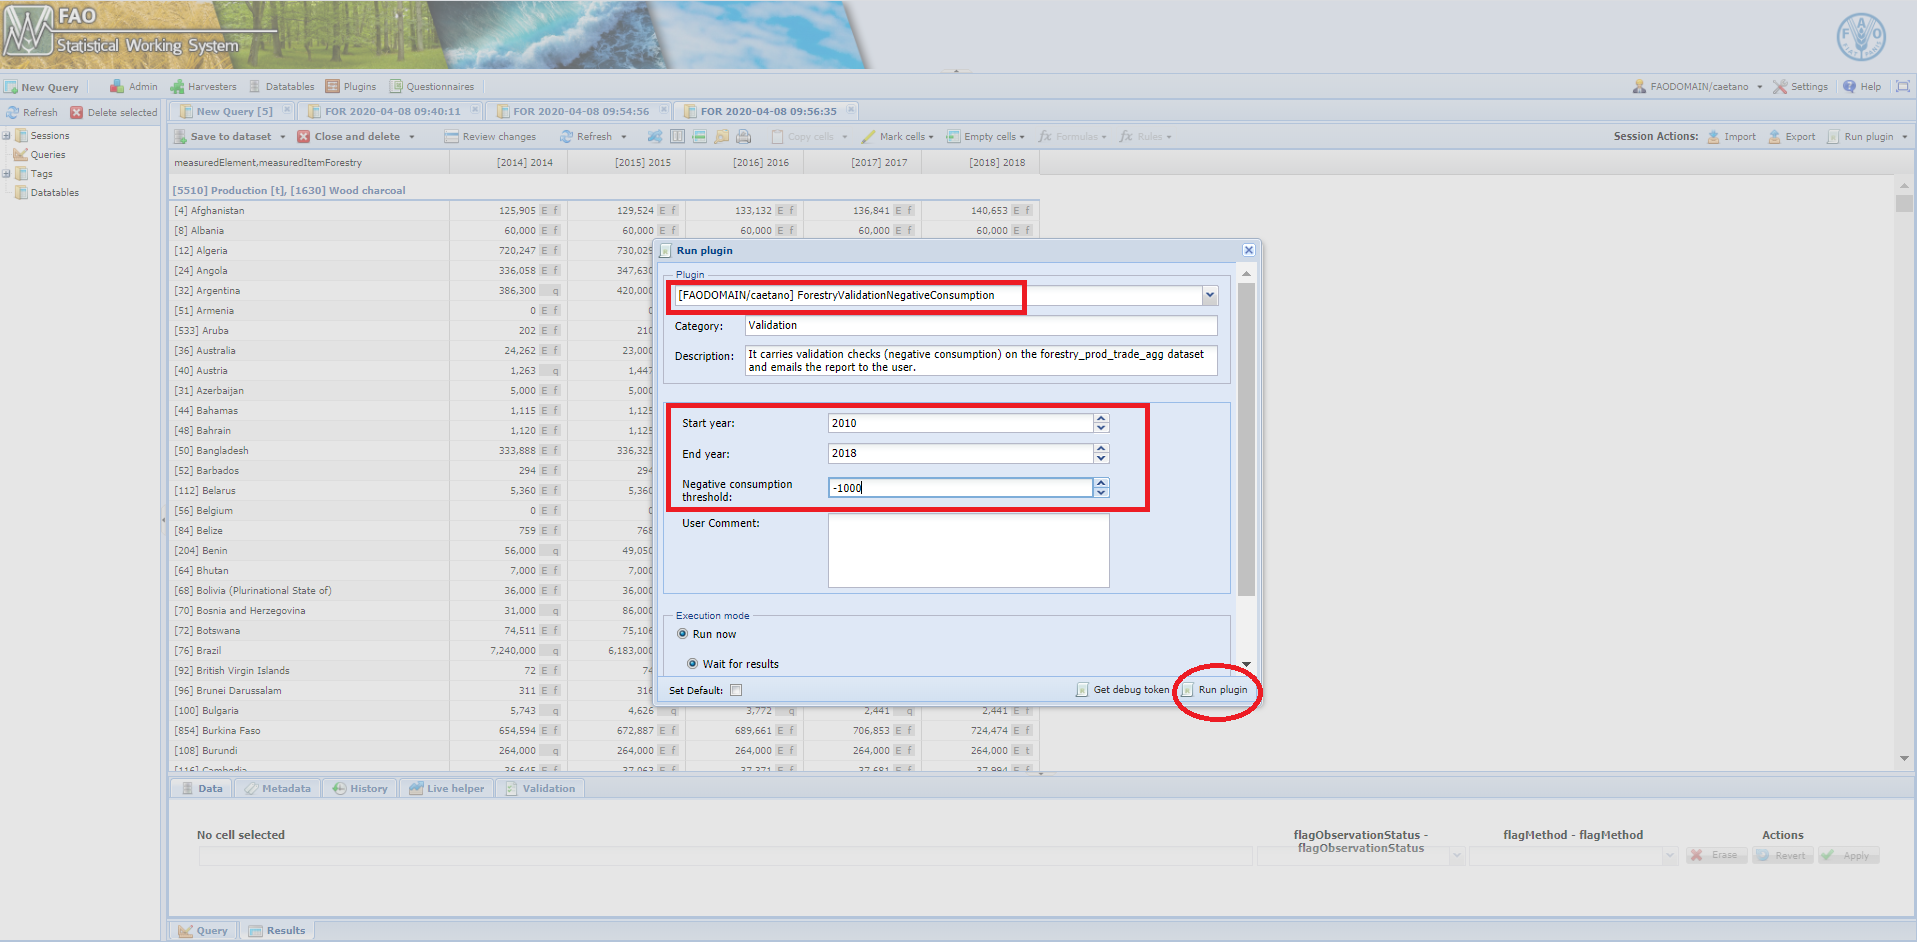
\includegraphics[width=1\linewidth]{images/negative_comsumption_parameters} 

}

\caption{Select the ForestryValidationNegativeConsump plugin and run it}\label{fig:NegConsumpPlugin}
\end{figure}

6. Wait for a window message to appear in the session;

\begin{figure}

{\centering 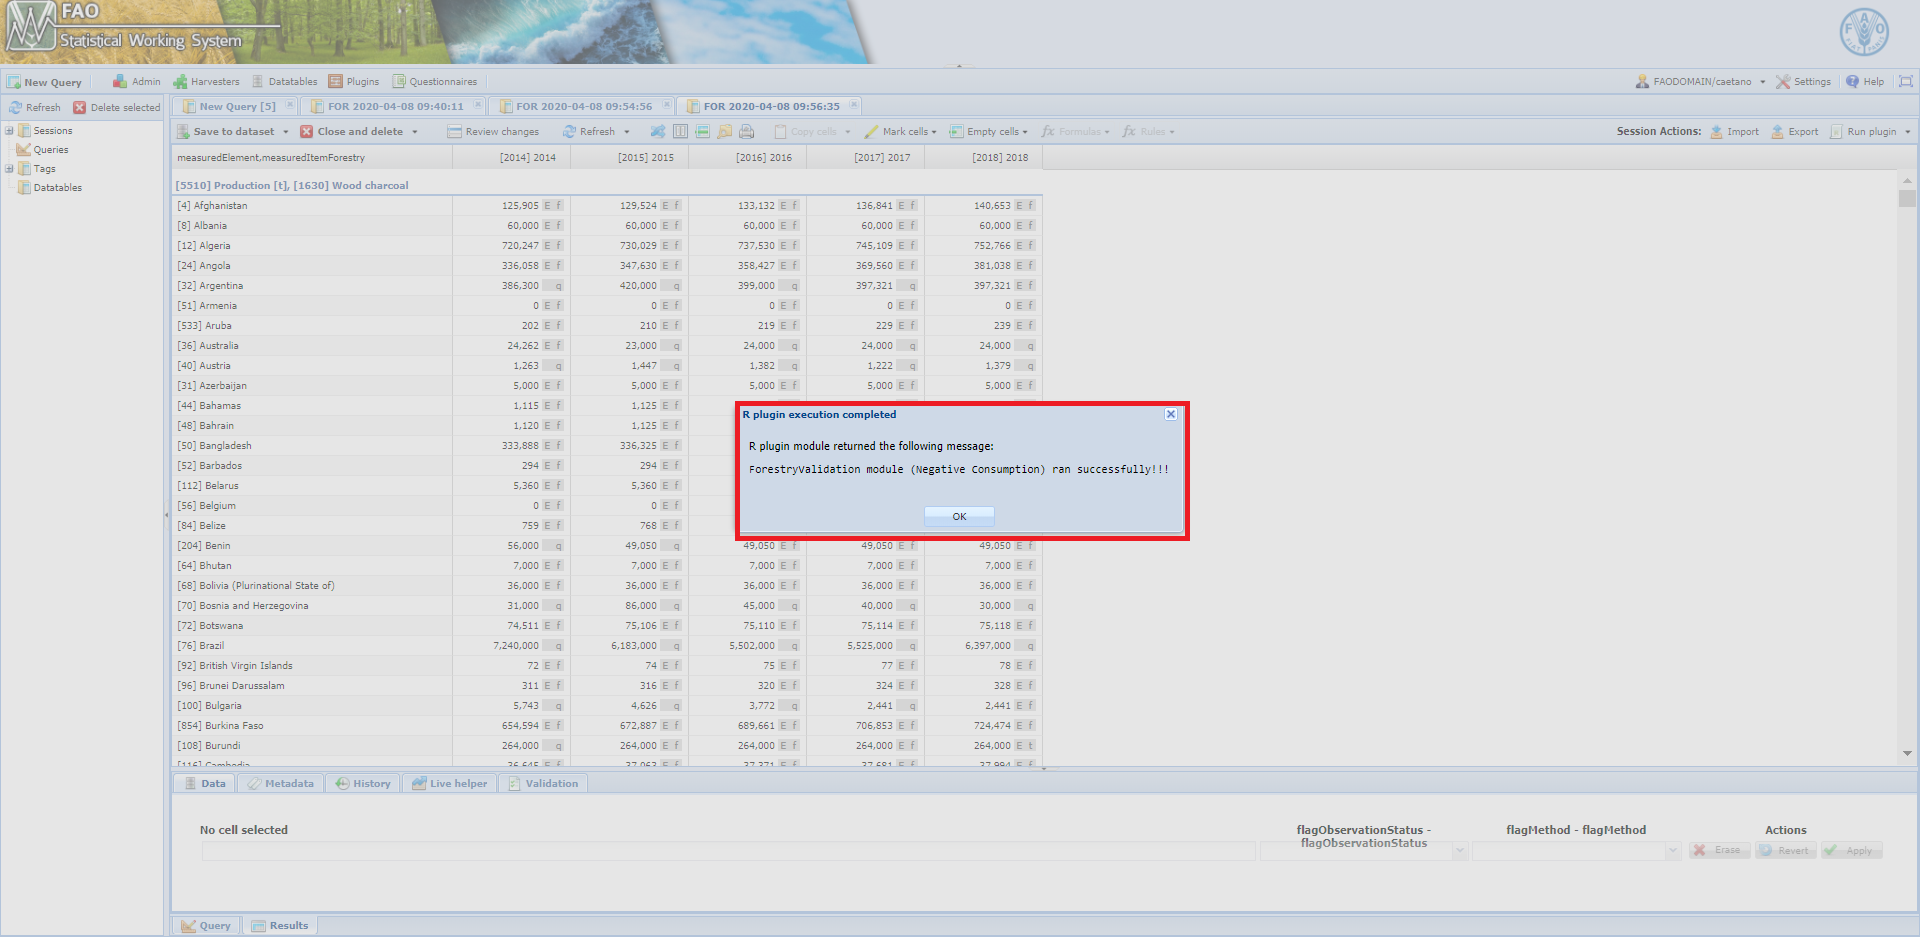
\includegraphics[width=1\linewidth]{images/negative_consump_message} 

}

\caption{ForestryValidationNegativeConsump module ran successfully}\label{fig:negConsumpPluginResults}
\end{figure}

\begin{enumerate}
\def\labelenumi{\arabic{enumi}.}
\setcounter{enumi}{6}
\tightlist
\item
  Get your results sent by email.
  \textbackslash begin\{figure\}
\end{enumerate}

\{\centering 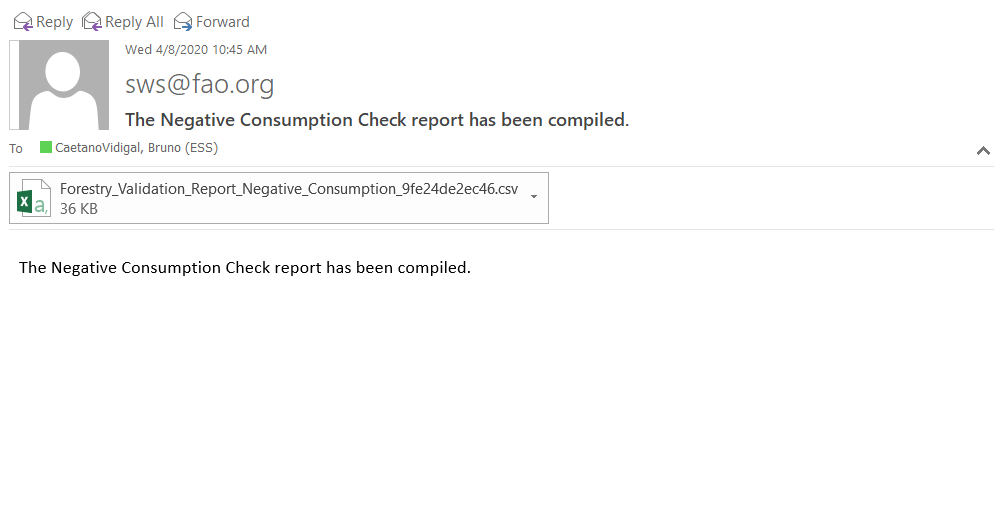
\includegraphics[width=0.8\linewidth]{images/negative_consump_email_sent}

\}

\caption{Email sent to the user with results}

\label{fig:NegConsumpPluginEmail}
\textbackslash end\{figure\}

\hypertarget{ForestryValidationUnitPrice}{%
\chapter{\texorpdfstring{\textbf{The ForestryValidationUnitPrice module}}{The ForestryValidationUnitPrice module}}\label{ForestryValidationUnitPrice}}

The module \textbf{ForestryValidationUnitPrice} pulls out records with significant abnormal high or low import/export unit price, given a threshold (\emph{quantity}) set by the user.

\begin{figure}

{\centering \includegraphics[width=1\linewidth]{images/ForestryValidationUnitPrice} 

}

\caption{Workflow of the ForestryValidationUnitPrice module}\label{fig:ForestryValidationUnitPriceWorkflow}
\end{figure}

\hypertarget{steps-6}{%
\section{\texorpdfstring{\textbf{Steps}}{Steps}}\label{steps-6}}

The module can be basically split into four parts as below.

\hypertarget{read-in-data-2}{%
\subsection{Read in data}\label{read-in-data-2}}

The module reads data from \textbf{forestry\_prod\_trade\_agg} dataset and from the datatables listed in the figure \ref{fig:ForestryValidationUnitPriceWorkflow}.

\hypertarget{data-filtering-2}{%
\subsection{Data filtering}\label{data-filtering-2}}

After pulling the needed data, the module applies filters using the parameters chosen by the user accordingly. The module has two kinds of parameters:

\begin{itemize}
\tightlist
\item
  time range (\emph{start} and \emph{end} year of the process) - \textbf{Start year} and \textbf{End year};
\item
  trade quantity threshold (minimum trade quantity analysed) - \textbf{Export Qty threshold} and \textbf{Import Qty threshold}.
\end{itemize}

\hypertarget{unit-price-check}{%
\subsection{Unit Price check}\label{unit-price-check}}

At this stage, there are only the target data as the time range and trade quantity threshold were applied. Therefore, the module verifies if within the remaining data there is any item with a unit price beyond its limits. Please, see the datatable \protect\hyperlink{trade-outlier-tresholds}{Trade outlier tresholds} for more information on the limits by each item or go access it in the SWS.

\hypertarget{email-the-user-2}{%
\subsection{Email the user}\label{email-the-user-2}}

The final step of this module is to email the user with two \emph{.csv} files - unit price for imports and exports.

\hypertarget{running-the-module-6}{%
\section{\texorpdfstring{\textbf{Running the module}}{Running the module}}\label{running-the-module-6}}

\begin{enumerate}
\def\labelenumi{\arabic{enumi}.}
\item
  Log in the SWS;
\item
  Click on \textbf{New Query};
\item
  Select \textbf{Forestry domain} and \textbf{forestry\_prod\_trade\_agg dataset};
\item
  Select whatever geographicAreaM49, measuredElement, measuredItemForestry and timePointYears. After that, run the query;
  \textbackslash begin\{figure\}
\end{enumerate}

\{\centering 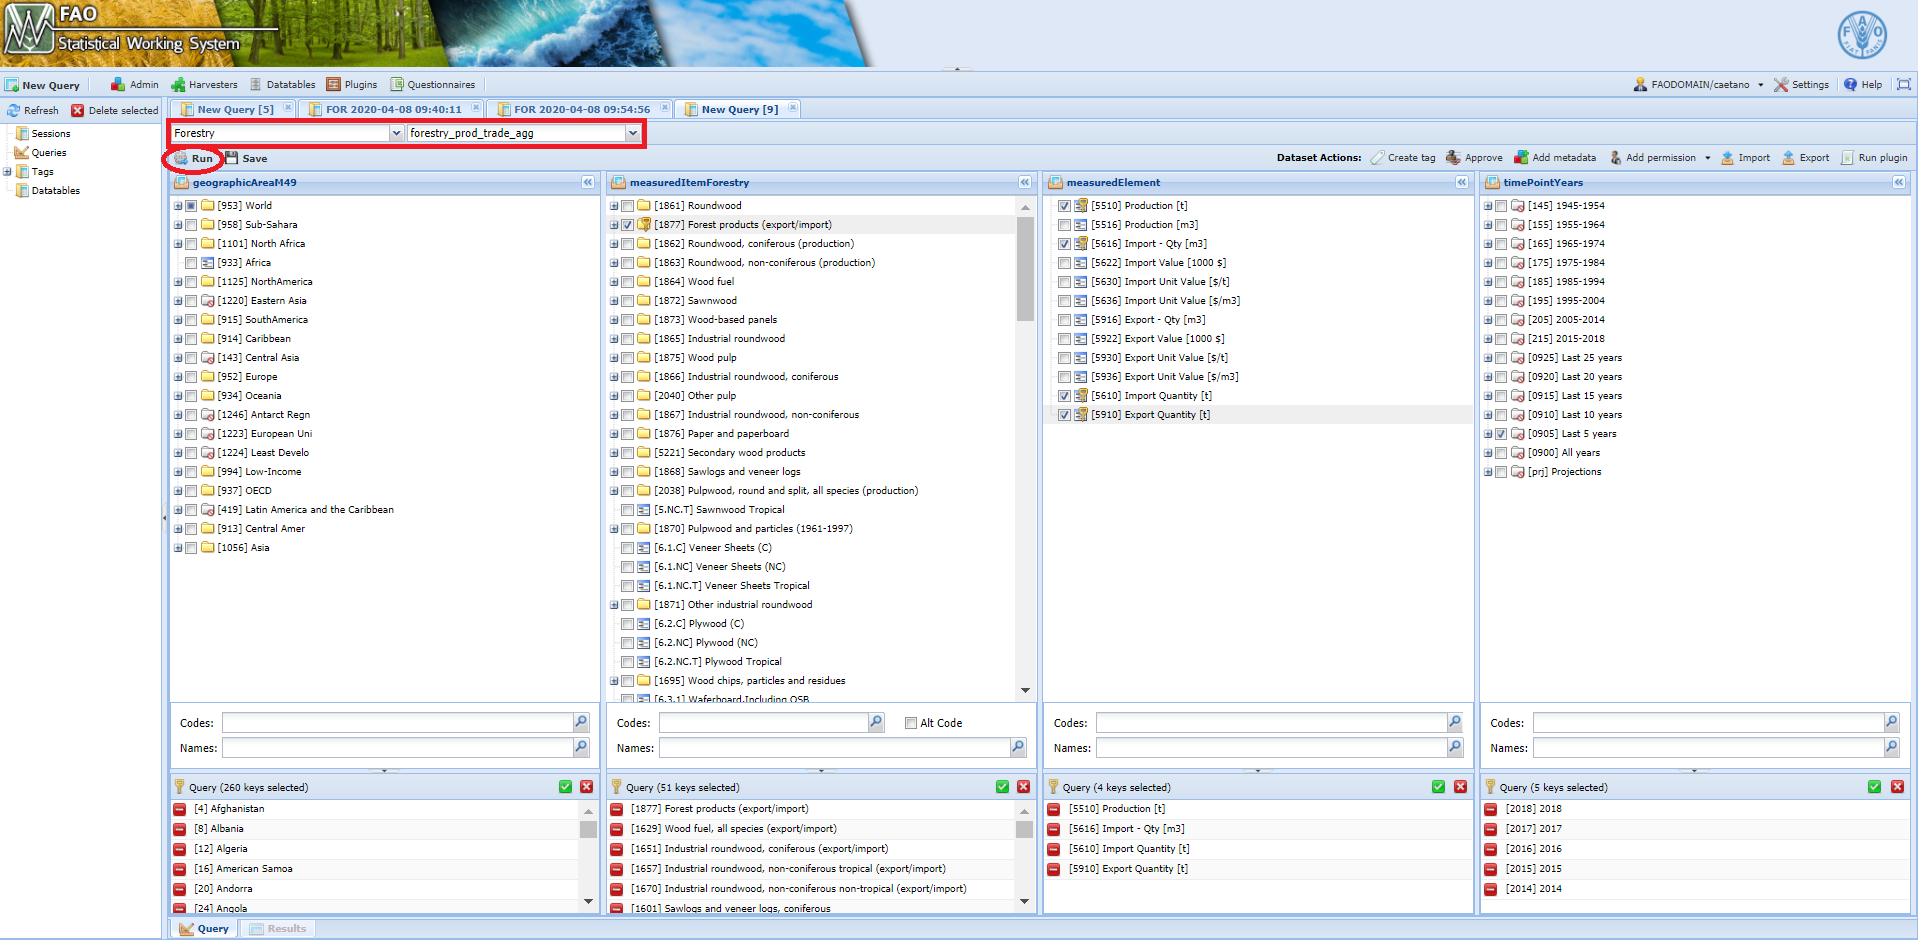
\includegraphics[width=1\linewidth]{images/forestry_prod_trade_agg_query}

\}

\caption{Steps 1 to 4}

\label{fig:queryUnitPrice}
\textbackslash end\{figure\}

\begin{enumerate}
\def\labelenumi{\arabic{enumi}.}
\setcounter{enumi}{4}
\tightlist
\item
  Select the \textbf{ForestryValidationUnitPrice} module, choose the \emph{parameters} (Start and End year ; Imports and Exports Quantity thresholds) and click on \textbf{Run plugin};
\end{enumerate}

\begin{figure}

{\centering 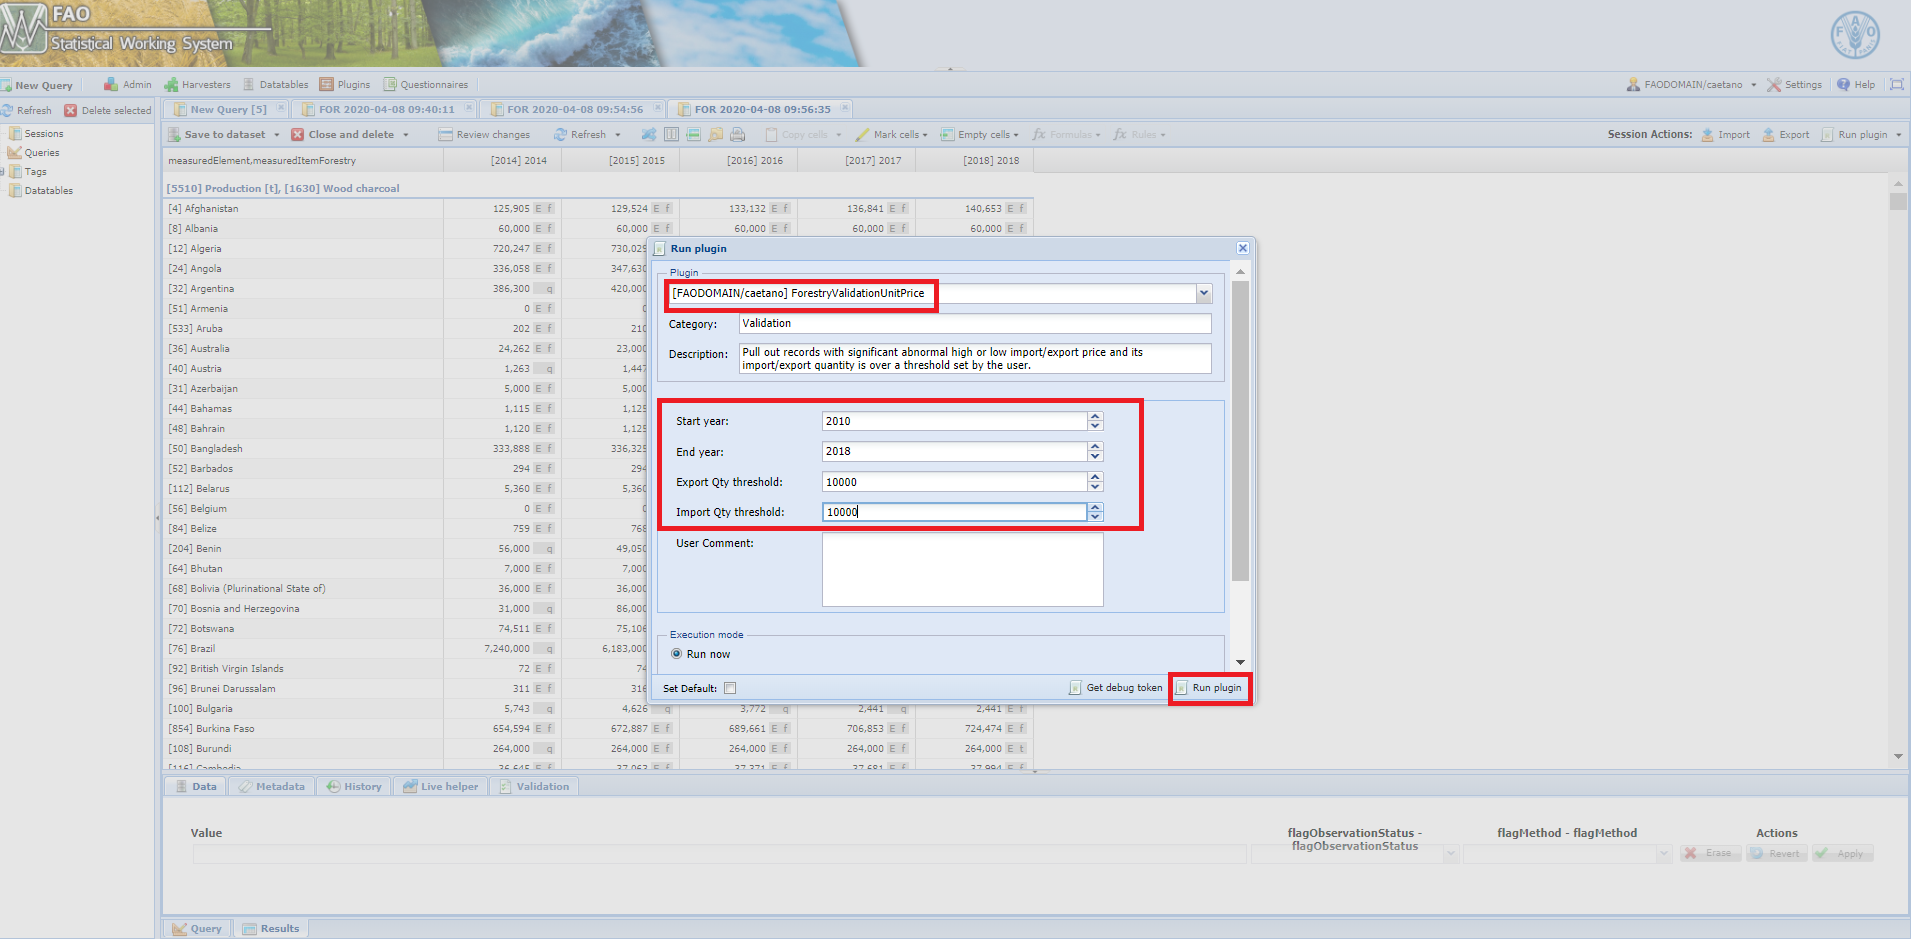
\includegraphics[width=1\linewidth]{images/forestry_select_plugin_unit_price} 

}

\caption{Select the ForestryValidationUnitPrice plugin and run it}\label{fig:UnitPricePlugin}
\end{figure}

6. Wait for a window message to appear in the session;

\begin{figure}

{\centering 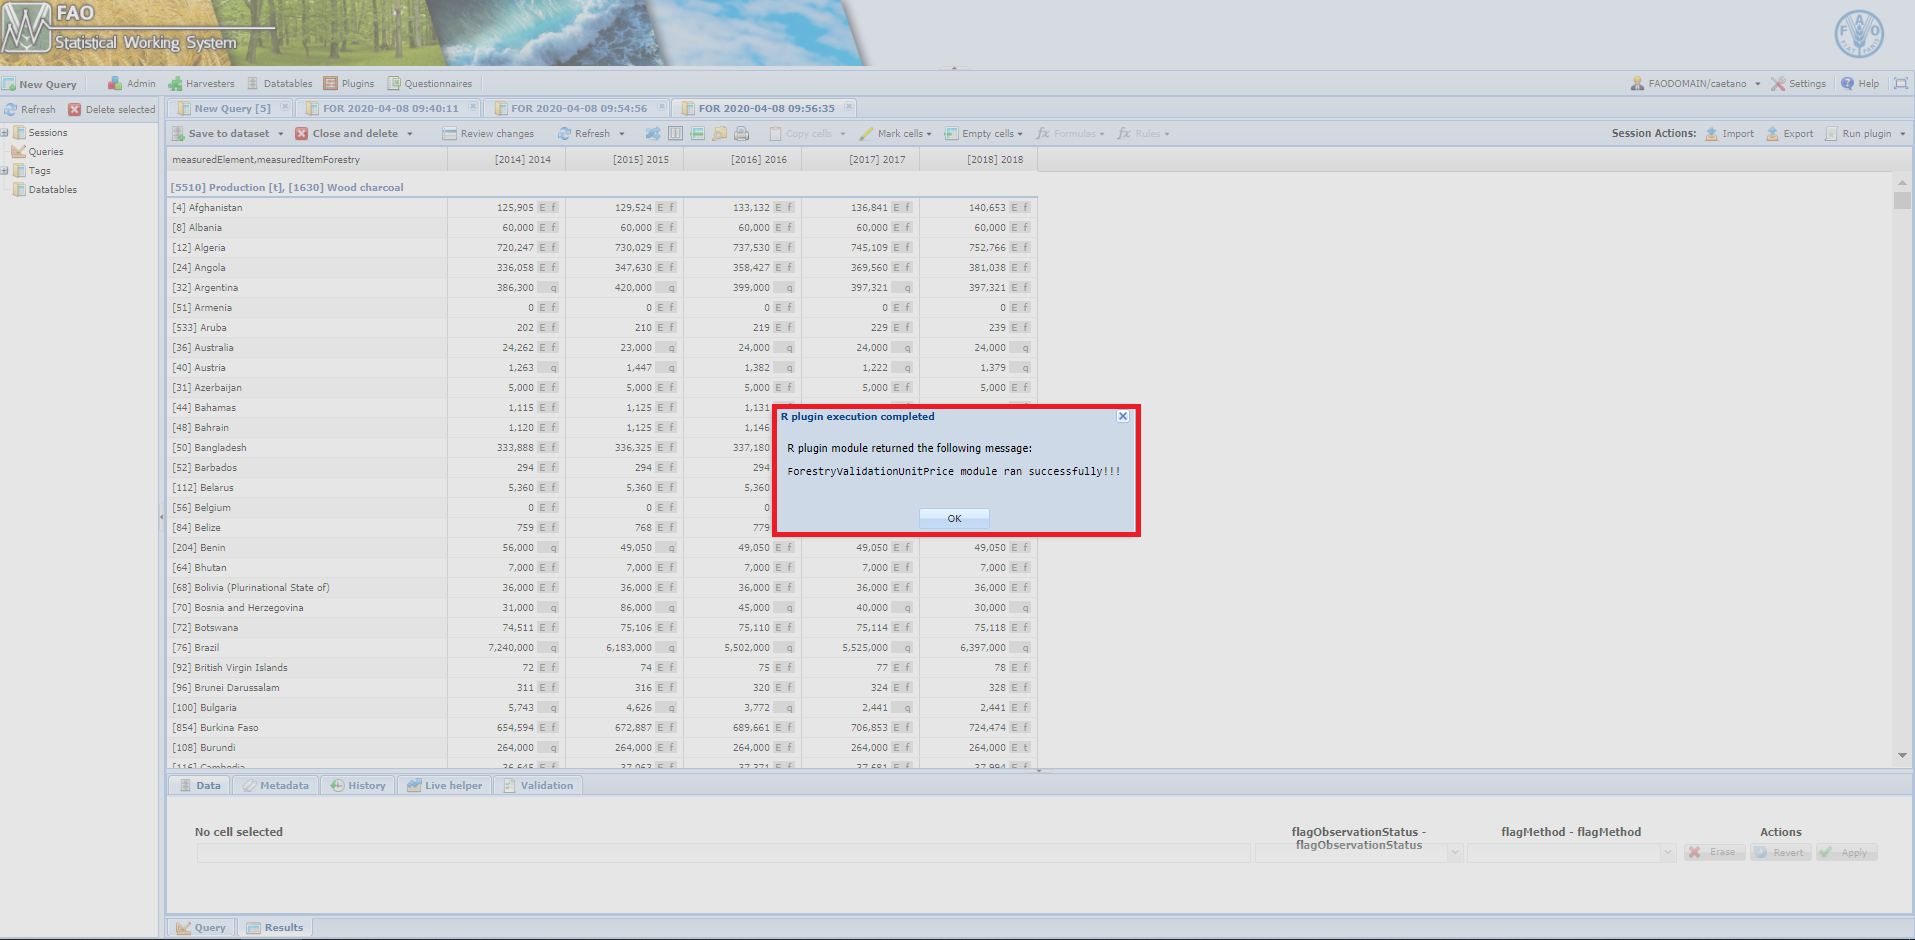
\includegraphics[width=1\linewidth]{images/result_unit_price_plugin} 

}

\caption{ForestryValidationUnitPrice module ran successfully}\label{fig:UnitPricePluginResults}
\end{figure}

\begin{enumerate}
\def\labelenumi{\arabic{enumi}.}
\setcounter{enumi}{6}
\tightlist
\item
  Get your results sent by email.
  \textbackslash begin\{figure\}
\end{enumerate}

\{\centering 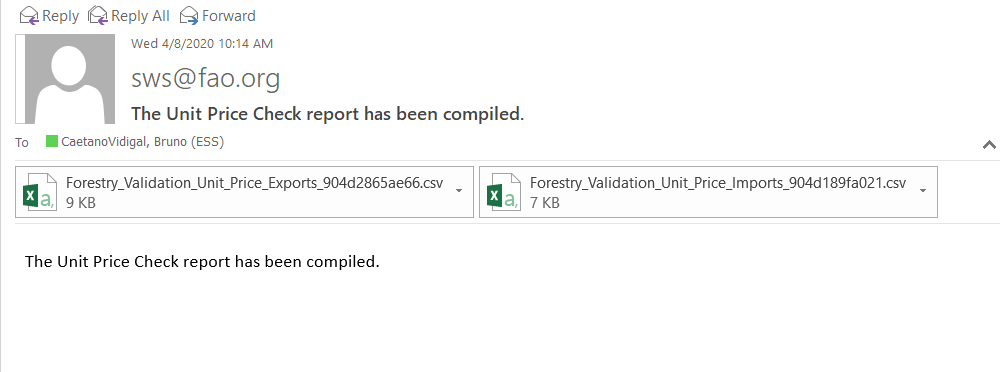
\includegraphics[width=0.8\linewidth]{images/unit_price_email_sent}

\}

\caption{Email sent to the user with results}

\label{fig:UnitPricePluginEmail}
\textbackslash end\{figure\}

\hypertarget{appendix-appendix}{%
\appendix}


\hypertarget{sws-resources}{%
\chapter{SWS resources}\label{sws-resources}}

SWS resources are R modules, datatables, data sets, and code lists comprising a migration framework. Datatables are typically used as auxiliary data to help R modules to achieve their goals. The statistical domains in SWS, through code/reference lists, define the dimensions of the datasets. Therefore, datasets are primarily used to store code list - referenced values as either input and output in the SWS.

\hypertarget{code-lists}{%
\section{Code lists}\label{code-lists}}

Code lists, also called reference lists in SWS parlance, are the dimensions making up the data sets that are designed by the user to store analytical results from SWS modules. The dimensions are statistical-domain-specific and are defined by the technical unit to reflect its needs regarding data collection, processing, and dissemination while meeting FAO standards. Each data set dimension has a set of codes and their associated descriptions. Thus, code lists serve to the purpose of standardization, visualization, and metadata by associating standardized codes to standardized names in the SWS data set outputs. A typical SWS compliant data set has, therefore, the following dimensions/reference lists:

\begin{itemize}
\item
  \textbf{Geographic area}. Representing a spatial scale the information is measured at. For example, countries, territories, regional aggregates, regional special groups aggregates, global aggregates. In SWS, the geographic area dimension used by Forestry Production and Trade data sets is named \textbf{geographicAreaM49}.
\item
  \textbf{Items}. Those one wants to take a measurement from. For example, commodities, commodity groups, land use types, species, etc. Typical item dimension names are \textbf{measuredItemCPC}, *\textbf{measuredItemHS}, \textbf{measuredItem}. In SWS, the item dimension used by Forestry Production and Trade data sets is named \textbf{measuredItemForestry}.
\end{itemize}

\begin{table}

\caption{\label{tab:measuredItemForestry}Forestry commodity codes in the measuredItemForestry code list.}
\centering
\fontsize{12}{14}\selectfont
\begin{tabular}[t]{lrlrlrlr}
\toprule
\rowcolor[HTML]{a9c9a7}  ItemName & ItemCode & ItemName & ItemCode & ItemName & ItemCode & ItemName & ItemCode\\
\midrule
Sawlogs and veneer logs, coniferous & 1601 & Recovered fibre pulp & 1609 & Builder's joinery and carpentry of wood & 1653 & Other fibreboard & 1650\\
Pulpwood, round and split, coniferous (production) & 1602 & Printing and writing papers, uncoated, wood containing & 1612 & Wooden furniture & 1658 & Industrial roundwood, coniferous (export/import) & 1651\\
Pulpwood, round and split, non-coniferous (production) & 1603 & Pulpwood, round and split, all species (export/import, 1961-1989) & 1614 & Prefabricated buildings & 1659 & Wooden wrapping and packaging material & 1652\\
Sawlogs and veneer logs, non-coniferous & 1604 & Printing and writing papers, uncoated, wood free & 1615 & Prefabricated buildings of wood & 1664 & Builder's joinery and carpentry of wood & 1653\\
OSB & 1606 & Printing and writing papers, coated & 1616 & Composite paper and paperboard & 1665 & Mechanical wood pulp & 1654\\
\addlinespace
Pulpwood and particles, coniferous (production, 1961-1997) & 1608 & Case materials & 1617 & Special coated paper and pulp products & 1666 & Semi-chemical wood pulp & 1655\\
Recovered fibre pulp & 1609 & Cartonboard & 1618 & Carbon paper and copying paper, ready for use & 1672 & Chemical wood pulp & 1656\\
Pulpwood and particles, non-coniferous (production, 1961-1997) & 1611 & Wood chips and particles & 1619 & Household and sanitary paper, ready for use & 1673 & Industrial roundwood, non-coniferous tropical (export/import) & 1657\\
Printing and writing papers, uncoated, wood containing & 1612 & Wood residues & 1620 & Packaging cartons, boxes etc. & 1677 & Wooden furniture & 1658\\
Printing and writing papers, uncoated, wood free & 1615 & Wrapping papers & 1621 & Other articles of paper and paperboard, ready for use & 1678 & Prefabricated buildings & 1659\\
\addlinespace
Printing and writing papers, coated & 1616 & Other papers mainly for packaging & 1622 & Printing and writing paper, ready for use & 1679 & Chemical wood pulp, sulphite, unbleached & 1660\\
Case materials & 1617 & Other industrial roundwood, coniferous (production) & 1623 & Articles, moulded or pressed from pulp & 1680 & Chemical wood pulp, sulphite, bleached & 1661\\
Cartonboard & 1618 & Sawnwood, non-coniferous tropical & 1624 & Filter paper and paperboard, ready for use & 1682 & Chemical wood pulp, sulphate, unbleached & 1662\\
Wood chips and particles & 1619 & Other industrial roundwood, all species (export/import, 1961-1989) & 1625 & Mechanical and semi-chemical wood pulp & 1685 & Chemical wood pulp, sulphate, bleached & 1663\\
Wood residues & 1620 & Other industrial roundwood, non-coniferous (production) & 1626 & Chemical wood pulp, sulphite & 1686 & Prefabricated buildings of wood & 1664\\
\addlinespace
Wrapping papers & 1621 & Wood fuel, coniferous & 1627 & Veneer sheets all & 1690 & Composite paper and paperboard & 1665\\
Other papers mainly for packaging & 1622 & Wood fuel, non-coniferous & 1628 & Wood products for domestic/decorative use & 1691 & Special coated paper and pulp products & 1666\\
Other industrial roundwood, coniferous (production) & 1623 & Wood fuel, all species (export/import) & 1629 & Other manufactured wood products & 1692 & Dissolving wood pulp & 1667\\
Sawnwood, non-coniferous tropical & 1624 & Wood charcoal & 1630 & Veneer sheets all, coniferous & 2065 & Pulp from fibres other than wood & 1668\\
Other industrial roundwood, non-coniferous (production) & 1626 & Sawnwood, coniferous & 1632 & Recovered post-consumer wood & 1600 & Recovered paper & 1669\\
\addlinespace
Wood fuel, coniferous & 1627 & Sawnwood, non-coniferous all & 1633 & Sawlogs and veneer logs, coniferous & 1601 & Industrial roundwood, non-coniferous non-tropical (export/import) & 1670\\
Wood fuel, non-coniferous & 1628 & Veneer sheets & 1634 & Pulpwood, round and split, coniferous (production) & 1602 & Newsprint & 1671\\
Wood charcoal & 1630 & Veneer sheets, coniferous & 1635 & Pulpwood, round and split, non-coniferous (production) & 1603 & Carbon paper and copying paper, ready for use & 1672\\
Sawnwood, coniferous & 1632 & Veneer sheets, non-coniferous all & 1637 & Sawlogs and veneer logs, non-coniferous & 1604 & Household and sanitary paper, ready for use & 1673\\
Sawnwood, non-coniferous all & 1633 & Veneer sheets, non-coniferous tropical & 1638 & OSB & 1606 & Printing and writing papers & 1674\\
\addlinespace
Veneer sheets & 1634 & Plywood, coniferous & 1639 & Pulpwood and particles, coniferous (production, 1961-1997) & 1608 & Other paper and paperboard & 1675\\
Veneer sheets, coniferous & 1635 & Plywood & 1640 & Recovered fibre pulp & 1609 & Household and sanitary papers & 1676\\
Veneer sheets, non-coniferous all & 1637 & Plywood, non-coniferous all & 1641 & Pulpwood and particles, non-coniferous (production, 1961-1997) & 1611 & Packaging cartons, boxes etc. & 1677\\
Veneer sheets, non-coniferous tropical & 1638 & Plywood, non-coniferous tropical & 1642 & Printing and writing papers, uncoated, wood containing & 1612 & Other articles of paper and paperboard, ready for use & 1678\\
Plywood, coniferous & 1639 & Particle board and OSB (1961-1994) & 1646 & Pulpwood, round and split, all species (export/import, 1961-1989) & 1614 & Printing and writing paper, ready for use & 1679\\
\addlinespace
Plywood & 1640 & Hardboard & 1647 & Printing and writing papers, uncoated, wood free & 1615 & Articles, moulded or pressed from pulp & 1680\\
Plywood, non-coniferous all & 1641 & MDF/HDF & 1648 & Printing and writing papers, coated & 1616 & Wrapping and packaging paper and paperboard & 1681\\
Plywood, non-coniferous tropical & 1642 & Fibreboard, compressed (1961-1994) & 1649 & Case materials & 1617 & Filter paper and paperboard, ready for use & 1682\\
Particle board and OSB (1961-1994) & 1646 & Other fibreboard & 1650 & Cartonboard & 1618 & Other paper and paperboard n.e.s. & 1683\\
Hardboard & 1647 & Industrial roundwood, coniferous (export/import) & 1651 & Wood chips and particles & 1619 & Mechanical and semi-chemical wood pulp & 1685\\
\addlinespace
MDF/HDF & 1648 & Mechanical wood pulp & 1654 & Wood residues & 1620 & Chemical wood pulp, sulphite & 1686\\
Fibreboard, compressed (1961-1994) & 1649 & Semi-chemical wood pulp & 1655 & Wrapping papers & 1621 & Veneer sheets all & 1690\\
Other fibreboard & 1650 & Chemical wood pulp & 1656 & Other papers mainly for packaging & 1622 & Wood products for domestic/decorative use & 1691\\
Mechanical wood pulp & 1654 & Industrial roundwood, non-coniferous tropical (export/import) & 1657 & Other industrial roundwood, coniferous (production) & 1623 & Other manufactured wood products & 1692\\
Semi-chemical wood pulp & 1655 & Chemical wood pulp, sulphite, unbleached & 1660 & Sawnwood, non-coniferous tropical & 1624 & Wood pellets & 1693\\
\addlinespace
Chemical wood pulp & 1656 & Chemical wood pulp, sulphite, bleached & 1661 & Other industrial roundwood, all species (export/import, 1961-1989) & 1625 & Other agglomerates & 1694\\
Chemical wood pulp, sulphite, unbleached & 1660 & Chemical wood pulp, sulphate, unbleached & 1662 & Other industrial roundwood, non-coniferous (production) & 1626 & Particle board & 1697\\
Chemical wood pulp, sulphite, bleached & 1661 & Chemical wood pulp, sulphate, bleached & 1663 & Wood fuel, coniferous & 1627 & Veneer sheets all, non-coniferous all & 1698\\
Chemical wood pulp, sulphate, unbleached & 1662 & Dissolving wood pulp & 1667 & Wood fuel, non-coniferous & 1628 & Veneer sheets all, non-coniferous tropical & 1699\\
Chemical wood pulp, sulphate, bleached & 1663 & Pulp from fibres other than wood & 1668 & Wood fuel, all species (export/import) & 1629 & Veneer sheets all, coniferous & 2065\\
\addlinespace
Dissolving wood pulp & 1667 & Recovered paper & 1669 & Wood charcoal & 1630 & Pitprops C & 1605\\
Pulp from fibres other than wood & 1668 & Industrial roundwood, non-coniferous non-tropical (export/import) & 1670 & Sawnwood, coniferous & 1632 & Pitprops NC & 1607\\
Recovered paper & 1669 & Newsprint & 1671 & Sawnwood, non-coniferous all & 1633 & Pitprops Trade & 1610\\
Newsprint & 1671 & Printing and writing papers & 1674 & Veneer sheets & 1634 & Poles Piling Posts C & 1613\\
Printing and writing papers & 1674 & Other paper and paperboard & 1675 & Veneer sheets, coniferous & 1635 & Wood for Charcoal & 1631\\
\addlinespace
Other paper and paperboard & 1675 & Household and sanitary papers & 1676 & Veneer sheets, non-coniferous all & 1637 & Poles Piling Posts Trade & 1636\\
Household and sanitary papers & 1676 & Wrapping and packaging paper and paperboard & 1681 & Veneer sheets, non-coniferous tropical & 1638 & Fuelwood & 1684\\
Wrapping and packaging paper and paperboard & 1681 & Other paper and paperboard n.e.s. & 1683 & Plywood, coniferous & 1639 & Charcoal & 1687\\
Other paper and paperboard n.e.s. & 1683 & Mechanical and semi-chemical wood pulp & 1685 & Plywood & 1640 & Black Liquor & 1688\\
Mechanical and semi-chemical wood pulp & 1685 & Chemical wood pulp, sulphite & 1686 & Plywood, non-coniferous all & 1641 & Pitprop\&Oth Ind Roundwd & 5217\\
\addlinespace
Chemical wood pulp, sulphite & 1686 & Wood pellets & 1693 & Plywood, non-coniferous tropical & 1642 & Printing+Writing Paper & 5222\\
Wood pellets & 1693 & Other agglomerates & 1694 & Further processed sawnwood, coniferous & 1643 & Wrapg+Packg Paper+Board & 5223\\
Other agglomerates & 1694 & Particle board & 1697 & Further processed sawnwood, non-coniferous all & 1644 & Other Paper+Paperboard & 5224\\
Particle board & 1697 & Veneer sheets all, coniferous & 2065 & Further processed sawnwood, non-coniferous tropical & 1645 & Wood Charcoal & 5247\\
Veneer sheets all, coniferous & 2065 & Further processed sawnwood, coniferous & 1643 & Particle board and OSB (1961-1994) & 1646 & Chips and Particles & 5248\\
\addlinespace
Sawlogs and veneer logs, coniferous & 1601 & Further processed sawnwood, non-coniferous all & 1644 & Hardboard & 1647 & Wood Chips, Particles and Residues & 5249\\
Sawlogs and veneer logs, non-coniferous & 1604 & Further processed sawnwood, non-coniferous tropical & 1645 & MDF/HDF & 1648 & Recovered Paper & 5252\\
OSB & 1606 & Wooden wrapping and packaging material & 1652 & Fibreboard, compressed (1961-1994) & 1649 & Chemical Wood Pulp & 5503\\
\bottomrule
\end{tabular}
\end{table}

\begin{itemize}
\item
  \textbf{Elements}. Often representing a measurement that can be taken across different items. For example, area, production, share. In SWS, the element dimension/code list used by Forestry Production and Trade is \textbf{measuredElement}.
\item
  \textbf{Time} (the time unit the data is displayed for: year, months, etc). In SWS, the time dimension used by Forestry Production and Trade data sets is named \textbf{timePointYears}.
\item
  \textbf{Flag} (A standardized label indicating origin and/or nature of a number in the data set, e.g.~ (Official number)). In SWS, the flag dimension used by AQUASTAT data sets is named \textbf{flagObservationStatus}. Please check the \href{http://intranet.fao.org/statistics_coordination_portal/standards_for_quality_compliance/}{OCS statistical standards} and the \href{http://intranet.fao.org/fileadmin/user_upload/scp/Standards_for_quality_compliance/SSS_Observation_Status_Codes__Flags__endorsed__December_2016_.pdf}{flags document} to understand the flagObservationStatus rational and obtain the description of flags.
\end{itemize}

\begin{table}

\caption{\label{tab:tabFlagObservationStatus}Observation Status Flags Annotations}
\centering
\fontsize{14}{16}\selectfont
\begin{tabular}[t]{l|l|l}
\hline
\rowcolor[HTML]{a9c9a7}  Flag & Description & Annotation\\
\hline
<blank> & Official figure & Observation reported to FAO by official statistical government agencies.\\
\hline
B & Time series break & Break observations are characterized as such whendifferent content exist or a different methodology has beenapplied to this observation as compared with the preceding one (the one given for the previous period).\\
\hline
E & Estimated value & Observation obtained through an estimation methodology (e.g. to produce back-casts) or based on the use of a limited amount of data or ad hoc sampling and through additional calculations (e.g. to produce a value at an early stage of the production stage while not all data are available). It may also be used in case of experimental data (e.g. in the context of a pilot ahead of a full scale production process) or in case of data of (anticipated/assessed) low quality. If needed, additional (uncoded) information can be provided through (free text) “comments” at the observation level or at a higher level.\\
\hline
F & Forecast value & Value deemed to assess the magnitude which a quantity will assume at some future point of time (as distinct from ""estimated value"" which attempts to assess the magnitude of an already existent quantity).\\
\hline
I & Imputed value & Observation imputed by FAO to replace or fill gaps in national data series, in line with the recommendations of the Committee for the Coordination of Statistical Activities (CCSA).\\
\hline
O & Missing value & This code is to be used when no distinction is made between the reasons why data are missing. Data can be missing due to various reasons: data do not exist, are insignificant (or not collected because they are below a certain threshold), are unreliable, are not relevant for the period, or other reason not elsewhere specified.\\
\hline
M & Missing value (data cannot exist, not applicable) & Used to denote empty cells resulting from the impossibility to collect a statistical value (e.g. a particular education level or type of institution may be not applicable to a given country's education system).\\
\hline
Q & Missing value; suppressed & Used when data are suppressed due to statistical confidentiality considerations.\\
\hline
N & Not significant (negligible) & An observation is below the unit precision level.\\
\hline
P & Provisional value & An observation is characterized as “provisional” when the source agency –while it bases its calculations on its standard production methodology –considers that the data, almost certainly, are expected to be revised.\\
\hline
R & Revised & Revised official figure.\\
\hline
S & Exceptional event & Exceptional events such as earthquake, massive forest fire, draught and flooding that occurred in the corresponding period that may have affected the observation or caused a missing value.\\
\hline
T & Unofficial figure & Observation reported by non-official or semi-official sources. Includes semi-official figure. Includes data from trade organizations (e.g. International Grain Council, International Sugar Organization etc.).\\
\hline
X & Figure from international organizations & Observations, both official and non-official, reported by governmental international organizations (e.g. UN, ILO, WB, UNESCO, Eurostat etc. specification on which international organization is provided in the metadata).\\
\hline
\end{tabular}
\end{table}

- \textbf{Method} (A standardized label indicating method utilized to obtain a number in the data set. In SWS, the method dimension used by AQUASTAT data sets is named \textbf{flagMethod}. Please check the \href{http://intranet.fao.org/statistics_coordination_portal/standards_for_quality_compliance/}{OCS statistical standards} and the \href{http://intranet.fao.org/fileadmin/user_upload/scp/Standards_for_quality_compliance/SSS_Observation_Status_Codes__Flags__endorsed__December_2016_.pdf}{flags document} to understand the flagMethod rational and obtain the description of flags.

\begin{table}

\caption{\label{tab:tabFlagMethod}Method flags}
\centering
\fontsize{14}{16}\selectfont
\begin{tabular}[t]{l|l}
\hline
\rowcolor[HTML]{a9c9a7}  Flag & Description\\
\hline
- & Unknown collection method\\
\hline
b & Balancing item\\
\hline
c & Copied from elsewhere in the working system\\
\hline
e & Estimate automatically generated by a statistical algorithm (short: statistical estimate)\\
\hline
f & Estimate manually derived, also on the basis of expert judgement (short: manual estimate)\\
\hline
h & Collected using automatic data harvesting\\
\hline
i & Calculated as identity (e.g. yield)\\
\hline
n & Value not collected or estimated, but can be assumed to be negligible\\
\hline
p & Collected (manually) from publications or databases\\
\hline
q & Collected via a questionnaire (e.g. APQ)\\
\hline
s & Calculated as sum (e.g. Grand Total, or High-income countries)\\
\hline
t & Carry-forward estimate\\
\hline
u & Value not known\\
\hline
\end{tabular}
\end{table}

The Forestry flags were mapped out into the SWS flag system as below:

\begin{table}

\caption{\label{tab:flagMappedOut}FAOSTAT-SWS mapping for observations and methods in Forestry.}
\centering
\fontsize{12}{14}\selectfont
\begin{tabular}[t]{lll}
\toprule
\rowcolor[HTML]{a9c9a7}  flagFAOSTAT & flagObservationStatus & flagMethod\\
\midrule
F & E & f\\
W & X & p\\
X & T & p\\
Q & blank & q\\
Fp & F & t\\
\addlinespace
Fc & E & i\\
Ft & E & t\\
Fb & E & dash\\
q & blank & q\\
f & E & f\\
\addlinespace
x & T & p\\
w & X & p\\
\bottomrule
\end{tabular}
\end{table}

\begin{figure}

{\centering 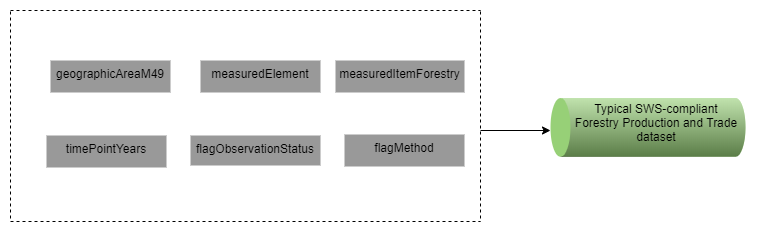
\includegraphics[width=0.65\linewidth]{images/typical_dataset_forestry} 

}

\caption{Typical dimensions (SWS code/reference lists) composing a Forestry Production and Trade SWS - compliant input/output dataset}\label{fig:fig4}
\end{figure}

\hypertarget{datatables}{%
\section{Datatables}\label{datatables}}

Datatables are mainly used to store information helping R modules to output analytical results. Information in datatables can be of a number of types. For example, conversion factors, arithmetic formulas, mapping between flags, mapping between international classifications, etc. In SWS hierarchy. all datatables reside in a given statistical domain.
Variable names (aka column names) in SWS datatables are more flexible in terms of the names they can take than SWS datasets. One can find SWS datatables naming variables as element\_code, element\_code\_sws, element\_code\_faostat, etc. Likewise, columns describing countries across different datatable may have different classification systems. This flexibility in datatables is beneficial as it allows to accommodate different auxiliary information.
In the AQUASTAT - SWS migration framework, the data tables are in the \textbf{Aquastat domain}. Below is a list of current available and filled data tables in the Aquastat domain.

\hypertarget{forestry-product-aggregation-elements}{%
\section*{Forestry Product Aggregation Elements}\label{forestry-product-aggregation-elements}}
\addcontentsline{toc}{section}{Forestry Product Aggregation Elements}

\begin{itemize}
\tightlist
\item
  \textbf{Datatable:} \texttt{Forestry\ Product\ Aggregation\ Elements}
\item
  \textbf{Domain:} Forestry
\item
  \textbf{Usage:}
\end{itemize}

\begin{table}

\caption{\label{tab:forestryproductaggregationelements}Columns description of the datatable: Forestry Product Aggregation Elements}
\centering
\fontsize{14}{16}\selectfont
\begin{tabular}[t]{l|l}
\hline
\rowcolor[HTML]{a9c9a7}  Field & Description\\
\hline
Group & Forestry item group\\
\hline
Element & Element from measuredElement code list\\
\hline
Aggregate & Flag of aggregate\\
\hline
Start Year & First year of the aggregate\\
\hline
End Year & Last year of the aggregate\\
\hline
\end{tabular}
\end{table}

\hypertarget{forestry-product-aggregation-tree}{%
\section*{Forestry Product Aggregation Tree}\label{forestry-product-aggregation-tree}}
\addcontentsline{toc}{section}{Forestry Product Aggregation Tree}

\begin{itemize}
\tightlist
\item
  \textbf{Datatable:} \texttt{Forestry\ Product\ Aggregation\ Tree}
\item
  \textbf{Domain:} Forestry
\item
  \textbf{Usage:} A datatable with group commodity and their primary commodities
\end{itemize}

\begin{table}

\caption{\label{tab:forestryproductaggregationtree}Columns description of the datatable: Forestry Product Aggregation Tree}
\centering
\fontsize{14}{16}\selectfont
\begin{tabular}[t]{l|l}
\hline
\rowcolor[HTML]{a9c9a7}  Field & Description\\
\hline
Group & Forestry item group\\
\hline
Commodity & Forestry item\\
\hline
Factor & \\
\hline
Aggr.Pass & \\
\hline
\end{tabular}
\end{table}

\hypertarget{forestry-aggregate-composition}{%
\section*{Forestry Aggregate Composition}\label{forestry-aggregate-composition}}
\addcontentsline{toc}{section}{Forestry Aggregate Composition}

\begin{itemize}
\tightlist
\item
  \textbf{Datatable:} \texttt{forestry\_aggregate\_composition}
\item
  \textbf{Domain:} Forestry
\item
  \textbf{Usage:}
\end{itemize}

\textbackslash begin\{table\}

\textbackslash caption\{\label{tab:forestryaggregatecomposition}Columns description of the datatable: forestry\_aggregate\_composition\}
\centering
\fontsize{14}{16}\selectfont

\begin{tabular}[t]{l|l}
\hline
\rowcolor[HTML]{a9c9a7}  Field & Description\\
\hline
item\_group\_code & Forestry item group code\\
\hline
item\_code & Forestry item code\\
\hline
agg\_order & Order of aggregation\\
\hline
first\_aggregates & First items to be aggregated\\
\hline
\end{tabular}

\textbackslash end\{table\}

\hypertarget{forestry-countries-partners}{%
\section*{Forestry Countries Partners}\label{forestry-countries-partners}}
\addcontentsline{toc}{section}{Forestry Countries Partners}

\begin{itemize}
\tightlist
\item
  \textbf{Datatable:} \texttt{forestry\_country\_partners}
\item
  \textbf{Domain:} Forestry
\item
  \textbf{Usage:}
\end{itemize}

\textbackslash begin\{table\}

\textbackslash caption\{\label{tab:forestrycountrypartners}Columns description of the datatable: forestry\_country\_partners\}
\centering
\fontsize{14}{16}\selectfont

\begin{tabular}[t]{l|l}
\hline
\rowcolor[HTML]{a9c9a7}  Field & Description\\
\hline
country & Country name\\
\hline
partner & Name of the Forestry partner\\
\hline
\end{tabular}

\textbackslash end\{table\}

\hypertarget{forestry-domain-elements}{%
\section*{Forestry Domain Elements}\label{forestry-domain-elements}}
\addcontentsline{toc}{section}{Forestry Domain Elements}

\begin{itemize}
\tightlist
\item
  \textbf{Datatable:} \texttt{forestry\_domain\_elements}
\item
  \textbf{Domain:} Forestry
\item
  \textbf{Usage:} An SWS datatable storing relevant Forestry elements and used to filter input dataset.
\end{itemize}

\textbackslash begin\{table\}

\textbackslash caption\{\label{tab:forestrydomainelements}Columns description of the datatable: forestry\_domain\_elements\}
\centering
\fontsize{14}{16}\selectfont

\begin{tabular}[t]{l|l}
\hline
\rowcolor[HTML]{a9c9a7}  Field & Description\\
\hline
domain\_code & Code of the Forestry domain\\
\hline
element\_code & Element code\\
\hline
element\_name & Element name\\
\hline
unit\_name & Unit of element\\
\hline
\end{tabular}

\textbackslash end\{table\}

\hypertarget{fs-m49-regions}{%
\section*{FS M49 regions}\label{fs-m49-regions}}
\addcontentsline{toc}{section}{FS M49 regions}

\begin{itemize}
\tightlist
\item
  \textbf{Datatable:} \texttt{fs\_m49\_regions}
\item
  \textbf{Domain:} Forestry
\item
  \textbf{Usage:}
\end{itemize}

\textbackslash begin\{table\}

\textbackslash caption\{\label{tab:fsm49regions}Columns description of the datatable: fs\_m49\_regions\}
\centering
\fontsize{14}{16}\selectfont

\begin{tabular}[t]{l|l}
\hline
\rowcolor[HTML]{a9c9a7}  Field & Description\\
\hline
fs\_reg & FAOSTAT area group code\\
\hline
m49\_reg & SWS area group code\\
\hline
group\_area\_name & Area group name\\
\hline
\end{tabular}

\textbackslash end\{table\}

\hypertarget{m49-fs-iso-mapping}{%
\section*{M49 FS ISO Mapping}\label{m49-fs-iso-mapping}}
\addcontentsline{toc}{section}{M49 FS ISO Mapping}

\begin{itemize}
\tightlist
\item
  \textbf{Datatable:} \texttt{m49\_fs\_iso\_mapping}
\item
  \textbf{Domain:} Common Domain
\item
  \textbf{Usage:} An SWS dataset datatable storing the mapping between FAOSTAT and UNSD M49 codes used to carry geographic aggregations.
\end{itemize}

\textbackslash begin\{table\}

\textbackslash caption\{\label{tab:m49fsisomapping}Columns description of the datatable: m49\_fs\_iso\_mapping\}
\centering
\fontsize{14}{16}\selectfont

\begin{tabular}[t]{l|l}
\hline
\rowcolor[HTML]{a9c9a7}  Field & Description\\
\hline
group\_area\_code & FAOSTAT group area code\\
\hline
group\_area\_name & Group area name\\
\hline
fs\_area\_code & FAOSTAT area code\\
\hline
fs\_area\_name & FAOSTAT area name\\
\hline
m49 & M49 area code\\
\hline
iso2 & ISO two-letter country code\\
\hline
iso3 & ISO three-letetr country code\\
\hline
\end{tabular}

\textbackslash end\{table\}

\hypertarget{trade-outlier-tresholds}{%
\section*{Trade outlier tresholds}\label{trade-outlier-tresholds}}
\addcontentsline{toc}{section}{Trade outlier tresholds}

\begin{itemize}
\tightlist
\item
  \textbf{Datatable:} \texttt{Trade\ outlier\ tresholds}
\item
  \textbf{Domain:} Forestry
\item
  \textbf{Usage:}
\end{itemize}

\begin{table}

\caption{\label{tab:Tradeoutliertresholds}Columns description of the datatable: Trade outlier tresholds}
\centering
\fontsize{14}{16}\selectfont
\begin{tabular}[t]{l|l}
\hline
\rowcolor[HTML]{a9c9a7}  Field & Description\\
\hline
item\_code & Forestry item code\\
\hline
element\_code & Element code\\
\hline
price\_lower & Lower price\\
\hline
price\_upper & Upper price\\
\hline
\end{tabular}
\end{table}

\hypertarget{uneceitto-input-data}{%
\section*{UNECE/ITTO Input Data}\label{uneceitto-input-data}}
\addcontentsline{toc}{section}{UNECE/ITTO Input Data}

\begin{itemize}
\tightlist
\item
  \textbf{Datatable:} \texttt{UNECE/ITTO\ Input\ Data}
\item
  \textbf{Domain:} Forestry
\item
  \textbf{Usage:} This datatable is an input for the \textbf{forestry\_prod\_trade} dataset. It contains the partner's data and it is used in the module Forestry\_UNECE\_ITTO\_Input\_Data. For more details check chapter \ref{ForestryUNECEITTOInputData}.
\end{itemize}

\begin{table}

\caption{\label{tab:uneceittoinputdata}Columns description of the datatable: UNECE/ITTO Input Data}
\centering
\fontsize{14}{16}\selectfont
\begin{tabular}[t]{l|l}
\hline
\rowcolor[HTML]{a9c9a7}  Field & Description\\
\hline
geographicAreaM49 & M49 country code\\
\hline
measuredItemForestry & Forestry item code\\
\hline
measuredElement & Element code\\
\hline
timePointYears & Year\\
\hline
DataValue & Value\\
\hline
flagObservationStatus & Flag of observation\\
\hline
flagMethod & Flag of method\\
\hline
MetadataValue\_Source & Source\\
\hline
\end{tabular}
\end{table}

\hypertarget{datasets}{%
\section{Datasets}\label{datasets}}

Datasets in the SWS are interchangeably used as module inputs/outputs and are composed by dimensions (aka reference/code lists). Because SWS datasets contain code lists following international standards as dimensions, there is little space for variation of dimension names across SWS datasets for the sake of standardization. The datasets in the Forestry domain are:

\begin{enumerate}
\def\labelenumi{\arabic{enumi}.}
\item
  \textbf{forestry\_prod\_trade}. The working dataset migrated from the current Input System into the SWS. \textbf{It is expected to be periodically manually edited by the technical unit (FOA) team. Changes made on this dataset may involve the domain-knowledge replacement of values due to arrival of new data at the end of data cycles and cell-level corrections via domain-knowledge}. Most importantly, after alterations, and if FOA wants so, this data set is used as \textbf{INPUT} to the \textbf{faoswsForestryAggregation} module. Details on the use of this dataset are in the (Chapter \ref{faoswsForestryAggregation}.
\item
  \textbf{forestry\_prod\_trade\_agg}. An SWS dataset serving as \textbf{output} of the \textbf{faoswsForestryAggregation}. It receives the geographic and commodity aggregations \textbf{after whatever saved change in the forestry\_prod\_trade data set}. Details on the use of this dataset are in the (Chapter \ref{faoswsForestryAggregation}.
\end{enumerate}

\end{document}
